\lstdefinelanguage{edma}%
  {
	morekeywords={[0]ValueDomain, on, Kind, DataModel, Relation, Singleton, Action, View, Unique, Equals, Compare, Integer, Long, Double, Float, String, Struct, Enum, OneOf, ListOf, Map, As, Publish, true, false, MIN, MAX, extends, Struct, Enum, OneOf, ListOf, Map, As, Publish, true, false, MIN, MAX, extends, Struct, Enum, OneOf, List, Map, As, Publish, true, false, MIN, MAX, extends, Extends, Constraints, Boolean, ?, +, >-<, >--, ---},
    sensitive=true,
	morecomment=[l]{//},
	morecomment=[s]{/*}{*/},
	morestring=[b]",
	showstringspaces=false
}%
\definecolor{keywordBlue}{rgb}{0,0,0.75}%
\definecolor{commentGreen}{rgb}{0,0.4,0}%
\definecolor{identifier}{rgb}{0.2,0.2,0.2}%
\lstset{xleftmargin=0.5cm,basicstyle=\small, tabsize=3}


\section{EDMA System Design}



The EDMA system consists of the following main components:
\begin{itemize}
\item A simple \emph{domain specific language} for defining value domains,
the structure of the data model and the interface for the data model\nomenclature[data model definition]{Data model definition}{A definition of a data model, ie. the elements that can be contained in a data model. A data model definition is often written in a Data Definition Language (DDL), opposed to a Data Manipulation Language (DML).}.
\item A \emph{compiler} to transform the definition files into an instance
of a \emph{meta model.}
\item A \emph{generator} that uses the \emph{meta model} instance to create: 

\begin{itemize}
\item An internal Java API for the data model that reflects the structure
of the data model. This API functions as an embedded DSL in java.
\item An external interface to the data model that applications can use
to communicate with the data model through.
\end{itemize}
\item A \emph{runtime system} used by the internal API to handle transaction
control and persistence.
\end{itemize}
The interface to the runtime system has been designed to allow flexibility
in the concrete implementations of the runtime system.

This means that different runtime systems can deploy different strategies
for transaction control, data storage and persistence and the user
can switch between different runtime systems without making any changes
to his code.

Figure \ref{fig:tobiasBilledeAfEdma} shows an overview of the EDMA
system.

\clearpage
\begin{figure}[h!]
\hspace{-1.5cm}
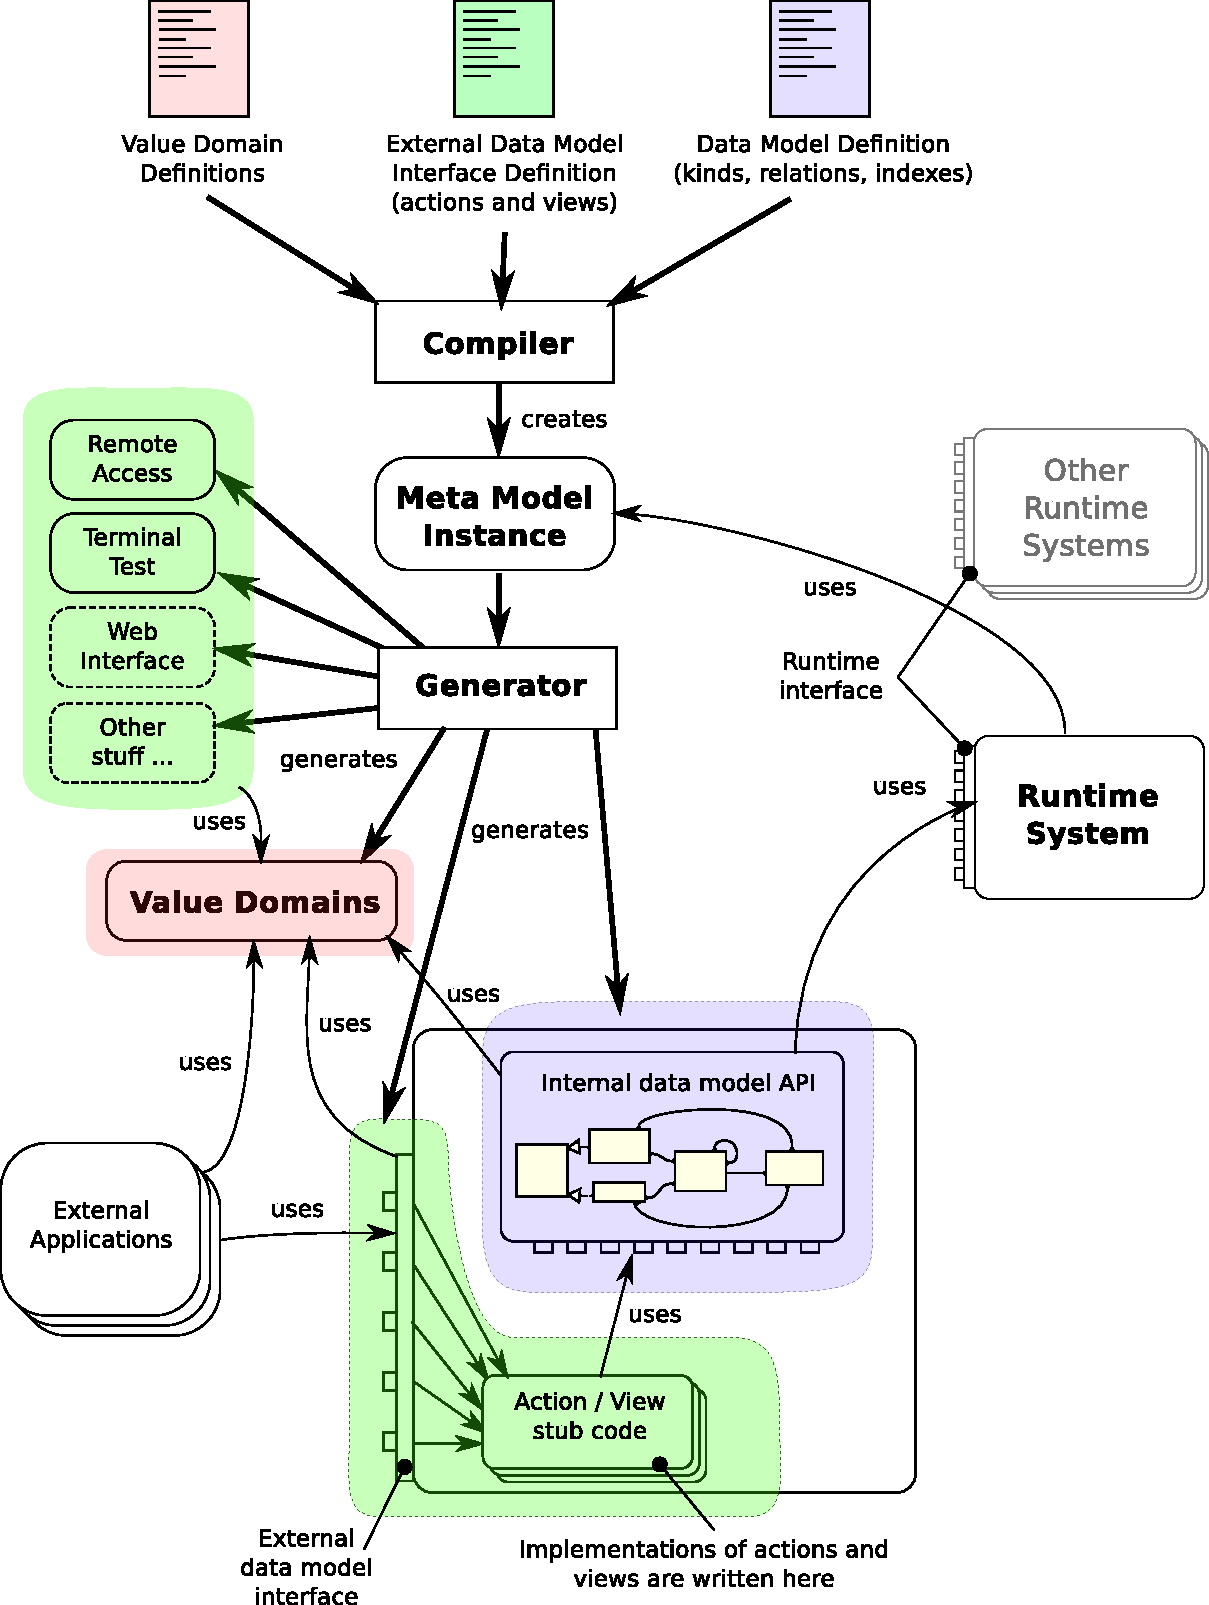
\includegraphics[width=\textwidth]{img/tobiasBilledeAfEdma.pdf}
\caption{Overview of the EDMA system. Definitions of value domains, data model external interface and data model structure are compiled into an instance of the meta model. The generator takes the meta model instance and generates model specific code including: Value domains, external data model interface and stub classes for implementing the methods in the external interface, an internal data model API that binds to the runtime system and various utility programs specialized to operate on the specific data model.}
\label{fig:tobiasBilledeAfEdma}
\end{figure}
\clearpage

We have taken an object oriented approach where the data model can
be seen as a class where the structure of the data model is encapsulated
from the outside world. The external interface of the data model is
the public part that external applications can use. As with classes
in object oriented languages, there can be several independent instances
of the same data model.

Each method in the external interface represents a transaction on
the data model. The semantic of the external interface is as if each
of these methods where synchronized on the same object. The individual
runtime system implementations may use more clever algorithms for
concurrency control, as long as the illusion of complete mutual exclusion
is kept intact. This analogy is used in order to keep focus on the
object oriented approach, instead of a traditional database approach.

The methods of the external interface are divided in two groups, \emph{views}
and \emph{actions}. Views cannot change the state of the data model
instance, only read it (this resembles const methods in C++). Actions
can both read and change the state of the instance.

In the following, we will describe the four main components in further
detail, starting with the meta model -- a very central element in
the EDMA system. Thereafter, we describe the compiler and the generator,
followed by a description of the example runtime system.


\subsection{\label{sub:Value-domains}Value Domains}

In most relational database systems, many different types of values
share the same data type. A person's name, an e-mail address, and
a URL could all have the same data type, e.g. \texttt{VARCHAR}. This
means that the type system is coarse grained, and it doesn't hinder
the user in storing, for example an e-mail, as a person's name.

In EDMA, we want to create a fine grained type system, where for example
an e-mail address, and a person's name belong to different types.
We call these types \emph{value domains}\nomenclature[value domain]{Value domain}{Can be seen as a type with extra restrictions on the possible values. Like the value 42 could be of type "int", the value "John" could be in a value domain "Name".}.

In EDMA we encourage the user to create a distinct value domain for
each semantically unique type. This not only adds useful semantic
information to the users of the value domains, it also makes the type
system able to discover a category of semantic errors, like if an
email address is accidentally used in place of a name or a URL.


\paragraph{Immutability}

In a multithreaded environment, mutable\nomenclature[mutable]{Mutable}{Changable. A mutable variable can get its value changed over the course of its lifetime.}
objects must be protected from race conditions, that can lead to threads
seeing them in an inconsistent state. For immutable\nomenclature[immutable]{Immutable}{Not changable. An immutable variable can never get its value changed over the course of its lifetime.}
objects this is not a problem, since they can never change after they
have been created. Therefore they will always be in a consistent state
(provided that they where created in a consistent state). Also, it
is never necessary to make defensive copies of immutable values, and
all values that are equal can be represented by the same instance.
For immutable values, the problem of accidental aliasing is also non-existing\cite{hogg1992geneva}.
For these reasons, in EDMA, all values (instances of value domains)
are immutable.


\paragraph{Value Domain Constraints}

The value domain system allows adding constraints to the value domains.
These constraints are automatically checked every time a new value
is created. As an example, the user can add a constraint to the value
domain \texttt{EmailAddress}, that checks that the content matches
a regular expression for accepted email addresses. 

There are two types of constraints on the value domains: \emph{Simple
constraints} and \emph{user implemented constraints}. The simple constraints
regard lengths and contents of strings, and numerical ranges for numeric
types. The user implemented constraints are, as the name suggests,
implemented by the user and can therefore be arbitrarily complex.

By defining constraints on the value domains the system can automatically
validate values when they are created.


\paragraph{Primitive Value Domains}

Value domains can be defined from the simple value domain types: \texttt{String},
\texttt{Integer}, \texttt{Long}, \texttt{Float}, \texttt{Double},
\texttt{Boolean} and \texttt{Enum}. Since we encourage the user to
create a fine-grained set of semantically unique value domains, the
primitive types can not be used directly, only in the definition of
other value domains.


\paragraph{Composed Value Domains}

It is possible to construct more complex value domains from the simpler
ones. For this purpose we have 3 different composable value domain
types: \texttt{Struct}, \texttt{List} and \texttt{OneOf}.


\paragraph{Struct}

The \texttt{Struct} value domain type consists of a number of attributes,
each of which has a name and a value domain. The struct value domain
type can therefore be seen as a container of multiple values, each
given a name. An example of a struct value domain, could be a \texttt{Date},
containing a \texttt{Day}, a \texttt{Month} and a \texttt{Year}. The
attributes in a struct value domain can be declared optional, which
means that the value might be \emph{null}.


\paragraph{List}

A \texttt{List} value domain type contains a number of values from
another value domain. For example, a value domain \texttt{NameList}
could be a list of \texttt{Name}s.


\paragraph{OneOf}

A \texttt{OneOf} value domain type contains a value from one of a
predefined set of value domains. An example could be a value domain
\texttt{Pet}, which can hold the value of either a \texttt{Dog}, \texttt{Cat},
or \texttt{Fish}. Thus the OneOf value domain type adds polymorphism
to the value domain system. 


\paragraph{Structurally Recursive Value Domains}

Value domains can be structurally recursive, meaning that for example
a value domain \texttt{Person} could contain a friend list of \texttt{Person}
values. But values (instances of value domains) are always tree-structures
and cannot contain loops or recursive references. In the above example
a person value cannot be in its own friend list. This is enforced
by the immutability of the values. It is only possible to construct
values from already created values, so all values are tree-structures
that are constructed in a bottom-up process. This means that it is
possible to define value domains where it would never be possible
to create a value from that value domain. 

An example would be a Struct value domain \emph{A} that contains a
field \emph{b} from value domain \emph{B} where the \emph{B} value
domain is a Struct containing a field \emph{a} from value domain \emph{A}.
You would need a value from value domain \emph{B} to create a value
from value domain \emph{A}, but to create a value from value domain
\emph{B} you need a value from value domain \emph{A}. One way to solve
this deadlock is to make at least one of the fields \emph{a} or \emph{b}
optional. The EDMA compiler will detect impossible value domains and
complain about them. This is done by checking that all recursive paths
contains an optional field, a list that may be empty or a OneOf with
a choice that breaks the loop.

There are advantages in having values that are guaranteed to be tree
structures and therefore self-contained and loop-free. This makes
processing values much simpler and the risk of entering an infinite
loop while processing values is greatly reduced. This also makes it
simple to move values across different borders of JVMs, machines,
languages etc.

It is worth to notice here that it \emph{is} possible to create a
value domain that represents a general graph by using indexes into
lists as references. However as long as the value domain contains
both the indexes and the lists they index into, this approach does
not break the self-contained and loop-free properties of the value
domain.


\paragraph{Expressiveness}

The value domain system is expressive enough to model itself as seen
in the following listing:

\begin{lstlisting}[basicstyle={\tiny},breaklines=true,tabsize=2]
ValueDomain MetaValueDomainSystem :
	List<MetaValueDomain> Constraints[noDuplicateOrMissingOrImpossible]
ValueDomain MetaValueDomain :
	Struct {name : UIdentifier, type : MetaValueDomainType, constraintList : ConstraintList}
ValueDomain MetaValueDomainType:
	OneOf<MetaPrimitiveType, MetaStructType, MetaListType, MetaOneOfType>
ValueDomain MetaPrimitiveType :
	OneOf<MetaStringType, MetaIntegerType, MetaFloatType, MetaBooleanType, MetaEnumType>
ValueDomain MetaStructType :
	List<MetaAttribute> Constraints[uniqueAttNames]
ValueDomain MetaAttribute :
	Struct {attName : LIdentifier, attValueDomain : UIdentifier, isOptional : TrueFalse}
ValueDomain MetaListType :
	Struct {elementValueDomain : UIdentifier, minLength : NotNegInt, maxLength : NotNegInt} Constraints[listMinLTEMax]
ValueDomain MetaOneOfType : List<UIdentifier>[1..MAX]
ValueDomain MetaStringType :
	Struct {minLength : NotNegInt, maxLength : NotNegInt, regexp? : Regexp} Constraints[stringMinLTEMax]
ValueDomain MetaIntegerType :
	Struct {min : AnyInt, max : AnyInt} Constraints[integerMinLTEMax]
ValueDomain MetaFloatType :
	Struct {min : AnyFloat, max : AnyFloat} Constraints[floatMinLTEMax]
ValueDomain MetaBooleanType :
	Struct {restrictedValue? : TrueFalse}
ValueDomain MetaEnumType : List<UIdentifier>

ValueDomain LIdentifier : String[1..MAX]["[a-z][A-Za-z0-9]*"]
ValueDomain UIdentifier : String[1..MAX]["[A-Z][A-Za-z0-9]*"]
ValueDomain TrueFalse : Boolean
ValueDomain AnyInt : Integer[MIN..MAX]
ValueDomain NotNegInt : Integer[0..MAX]
ValueDomain AnyFloat : Float[MIN..MAX]
ValueDomain Regexp : String[0..MAX]
ValueDomain ConstraintList : List<LIdentifier>
\end{lstlisting}


This makes it possible to create a value that represents a value domain
system for a specific domain, and use it as any other value in the
system e.g. use it in kind attributes, move it across socket connections
etc. It is also possible to model the meta model in the value domain
system, in this way an entire data model instance can be stored as
a single value.


\subsection{\label{sec:MetaModel}Meta Model}

The EDMA meta model is the central model that everything else in EDMA
is built around. The meta model is used to describe the individual
data models. An instance of the meta model represents a specific user
defined data model.

Since the meta model has many different elements, it is described
in a bottom-up fashion, starting with the most low-level definitions
first, gradually adding complexity as we go along.

%\begin{figure}[h]
%	\centering
%	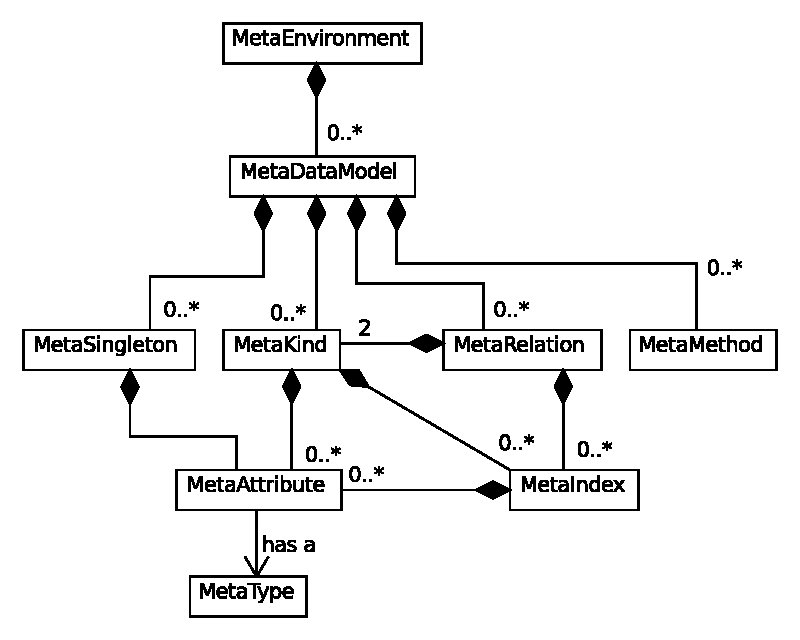
\includegraphics[width=0.75\textwidth]{img/metaModel.pdf}
%	\caption{The class diagram of the meta model is the %abstract syntax of the data model definition.}
%	\label{fig:metaModel}
%\end{figure}


\subsubsection{Kinds and Entities}

\begin{wrapfigure}{r}{0.4\textwidth}

	\begin{center}
		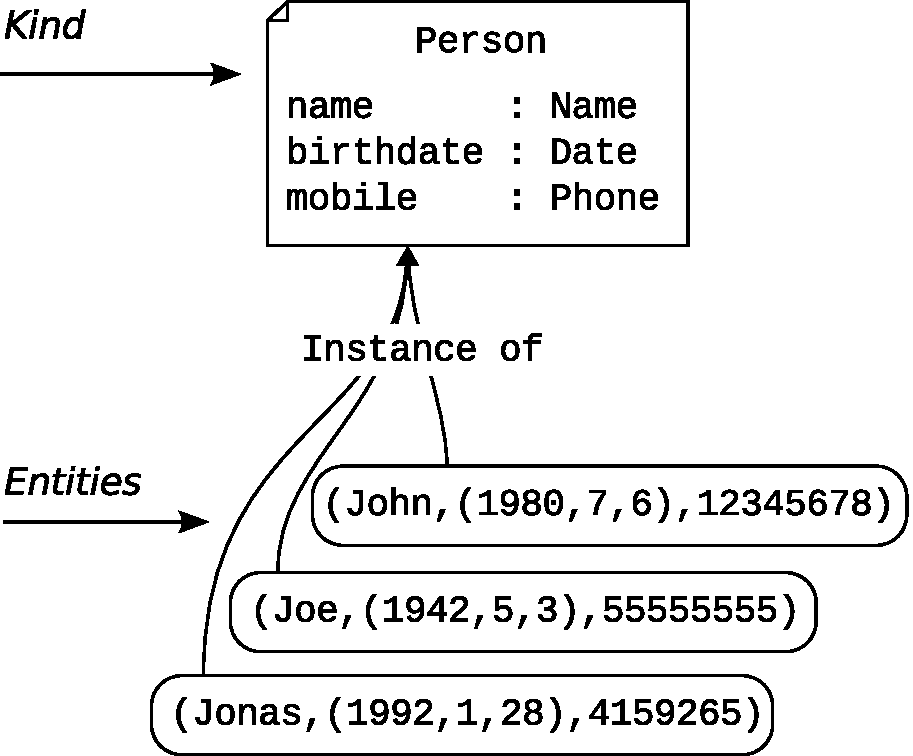
\includegraphics[width=0.4\textwidth]{img/kindAndEntities.pdf}
	\end{center}
	\caption{Kinds describe and contain entities, having certain attributes.}
	\label{fig:kindAndEntities}
\end{wrapfigure}

In EDMA a \emph{kind} \nomenclature[kind]{Kind}{A kind consists of a name and a set of attributes. An instance of a kind is called an entity. For example, a kind could be Person, with the attributes name, birth date and phone number. An entity of this kind could be (John, (1980, 3, 5), 31415926).}is
both a data type and a container of all instances of that type. A
kind has a set of \emph{attributes}\nomenclature[attribute]{Attribute}{A name and a value domain. An example could be "age" in the value domain "PositiveInteger", which is comparable to a variable "age" of type "uint". Attributes are either optional or mandatory, and mutable or immutable.},
where each attribute has a name and a value domain. An \emph{entity\nomenclature[entity]{Entity}{A set of values, conforming to a certain kind. }}
is an instance of a kind. As an example we could have a person kind
with attributes like name, gender, birth date, email and phone number.
A person entity would then contain a value for each of the attributes
in the person kind. Each attribute in a kind can be either mutable
or immutable. If it is immutable then a value for the attribute is
set upon creation of an entity, but this value can never change throughout
the lifetime of the entity. An attribute can be optional, which means
that the value corresponding to that attribute may be \emph{null}.
All kinds in EDMA have an attribute called ID, which is a positive
integer that uniquely identifies each \emph{entity} in the kind.


\subsubsection{Relations and Connections}

Assume that we have a person kind and a course kind, and we want to
be able to express that a person is a student on a course. In EDMA
we call this a \emph{relation\nomenclature[relation]{Relation}{A connection between two kinds. If a relation exists between kinds A and B, entities of A and B can be connected. For example, a relation can exist between kinds Course and Student, which means that an entity of course (eg. (Programming, 2012)) can be connected to a Student (eg. (John Doe, 1984, +4531415926)).}}
between the person kind and the course kind. When there is a \emph{relation}
between the person kind and the course kind, it is possible to make
a \emph{connection} between a specific person entity and a specific
course entity. A \emph{relation} is both a description of possible
\emph{connections} between entities and a container for these \emph{connections}.

\begin{figure}[h]
	\centering
	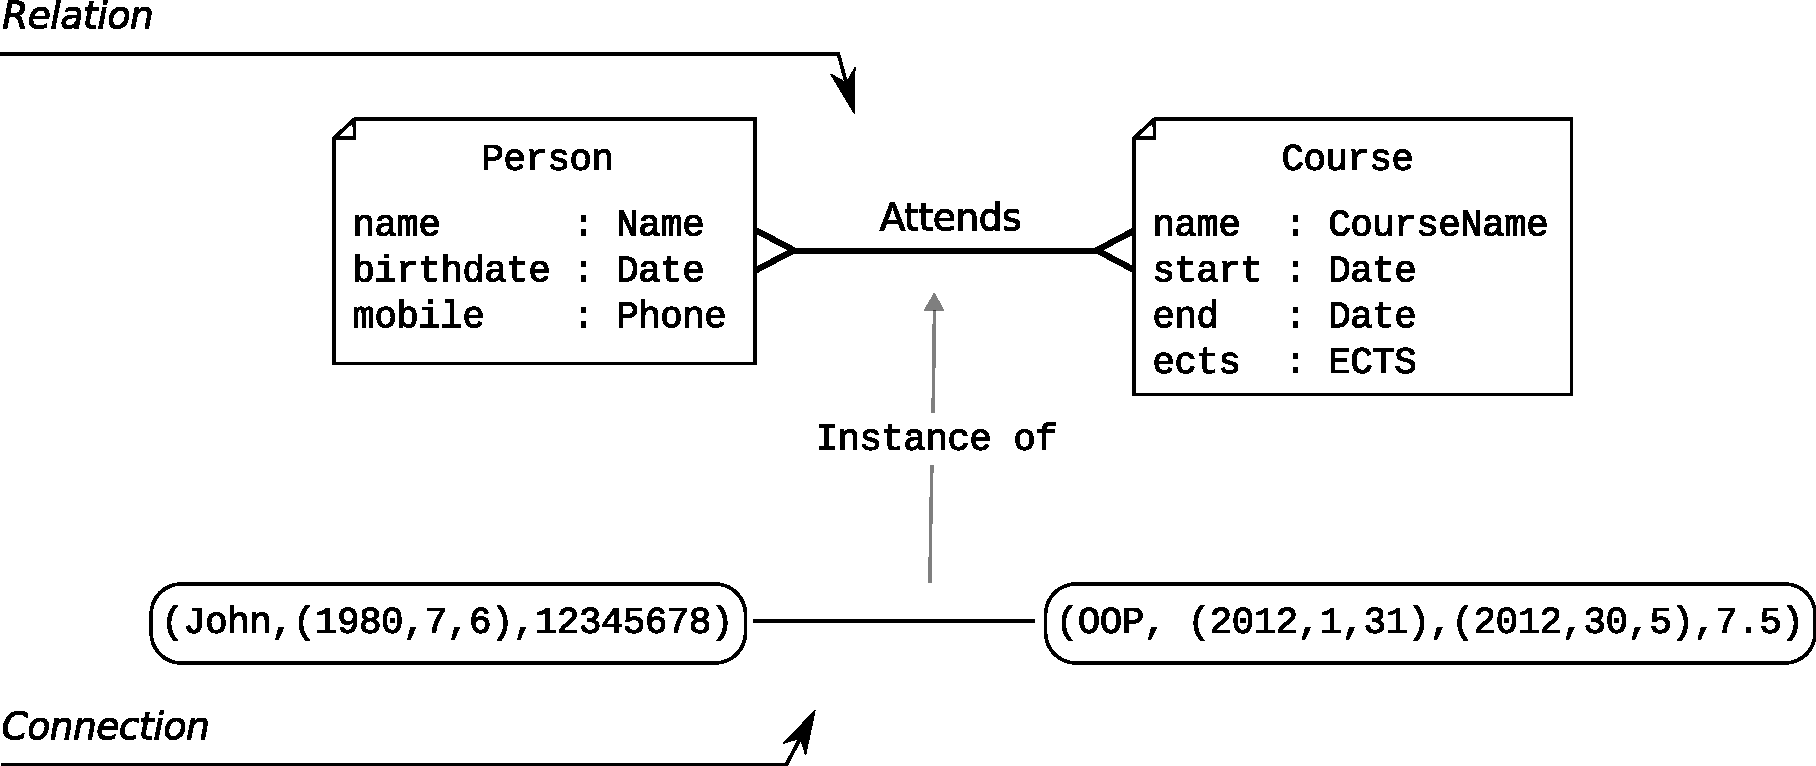
\includegraphics[scale=0.4]{img/relationAndConnection.pdf}
	\caption{A relation between two kinds makes it possible to \emph{connect} entities of those kinds.}
	\label{fig:relationAndConnection}
\end{figure}


\subparagraph{Roles}

A \emph{relation} always has two participants, which we can call A
and B. Both A and B are defined by a \emph{kind} and a \emph{role}.
The reason for having roles is that we can have different relations,
which involve the same kinds, in which case we use the roles to distinguish
them. In the example with the Person kind and the Course kind, we
could have two different relations between them: One that represents
students that are enrolled on the course, and one that represents
teachers that teach the course. To distinguish the two different \emph{relations},
the role of the person would be \emph{student} in the one relation,
and \emph{teacher} in the other. 

\begin{figure}[h]
	\centering
	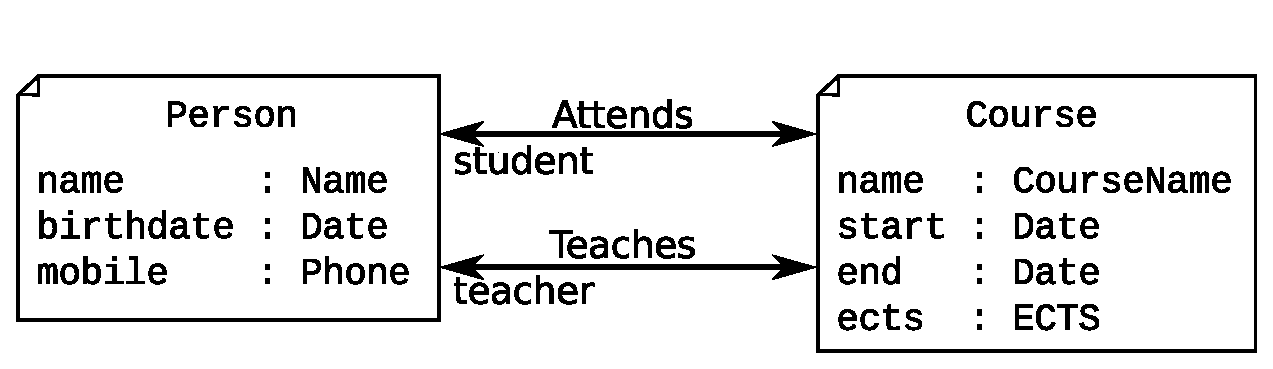
\includegraphics[width=0.75\textwidth]{img/relationRoles.pdf}
	\caption{A Relations between kinds can have roles. This figure shows two relations between the kinds Person and Course. In the first relation, named Attends, the first participant is the Person kind, with the role Student. In the second relation, Teaches, the Person has the role Teacher. In both Relations the second participant is the Course kind with the implicit role course.}
	\label{fig:relationRoles}
\end{figure}

It is also possible to have relations, where both the kind and the
role would be the same for A and B. An example could be a friendship
relation, where the kind is person and the role is friend for both
A and B, this type of relation we call a self-relation. If we have
a relation where A and B has the same kind, but different roles, then
it is not a self relation. An example of this could be where A and
B both are persons, but where the role of A is parent and the role
of B is child. In a self-relation, the order of the participants are
irrelevant, so if we have person a and person b, then ``a is friends
with b'' is the same as ``b is friends with a'', but there is a
difference between ``a is parent of b'' (or ``b is child of a'')
and ``b is parent of a'' (or ``a is child of b'').


\subparagraph{Multiplicities}

We also distinguish between many-to-many, many-to-one and one-to-one
relations (we do not have a one-to-many relation as this is the same
as a many-to-one where A and B are switched). It is worth to notice
that a many-to-one self-relation does not make any sense, so this
leaves us with five different types of relations:
\begin{enumerate}
\item Many-To-Many (MTM)
\item Many-To-Many-Self (MTMS)
\item Many-To-One (MTO)
\item One-To-One (OTO)
\item One-To-One-Self (OTOS)
\end{enumerate}
So, a relation in EDMA contains the following information: a name,
the kind of A, the role of A, the kind of B, the role of B, the type
of the relation (one of the five types above). If a role is not defined
on one of the participants, the role is set to the same as the name
of the participating kind. For example, in the relations shown on
Figure~\ref{fig:relationRoles}, the role of the Course is simply
``course''. In the five relation types above, \emph{many} actually
means \emph{0 or more} and \emph{one} actually means \emph{0 or 1}.

A \emph{connection} is an instance of a relation and can be thought
of as a set of pairs of ids (a, b). Each element in the set represents
the connection between an entity from kind A and an entity from kind
B with the ids a and b respectively. In a self-relation (a, b) is
the same as (b, a).


\subparagraph{Extension}

\begin{wrapfigure}{r}{0.3\textwidth}
	\vspace{-0.415cm}
	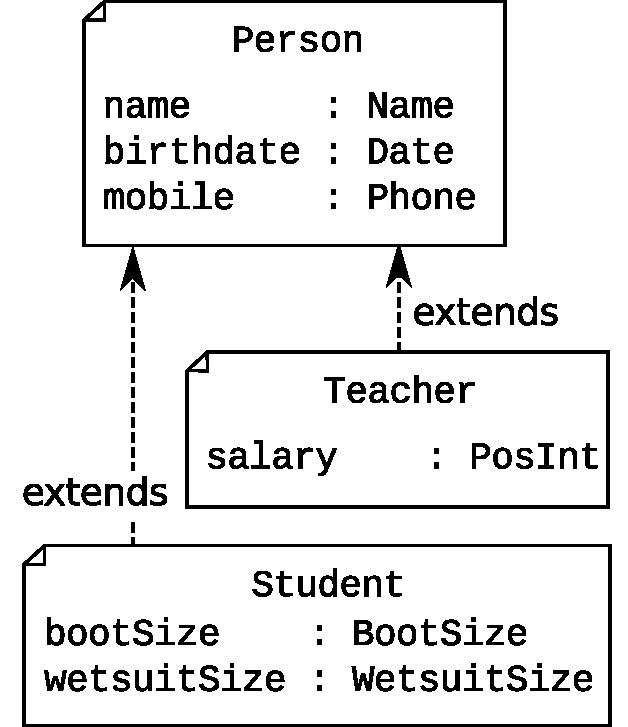
\includegraphics[width=0.3\textwidth]{img/kindExtension.pdf}
	\caption{Here, Student and Teacher extends Person, adding extra attributes.}
\end{wrapfigure}

There is actually a sixth relation type, which we call \emph{extension}.
An extension between kinds is a 1-to-(0 or 1) relation between two
different kinds. As an example we could have a kind, Person, and another
kind, Student, which extends Person. This means that every student
is also a person, so in order to create a new student, you would need
to provide an already existing person, that is not already a student.
We could also have another kind, Teacher, that also extends Person.
Then every teacher would also be a person, and a person could be both
a teacher and a student, or only one of them, or neither. In our running
example with the diving school, we have shown the kinds Student and
Teacher that both extend the kind Person.


\subsubsection{Indexes}

In EDMA indexes are used for two different purposes: To enforce uniqueness
of certain attributes within all entities of a kind, and to gain fast
and easy access to certain entities, or sets of entities. Indexes
can either be declared on a kind, in which case they cover all entities
of that kind, or they can be declared on a relation, in which case
they cover only sets of entities, that are grouped by that relation.
EDMA supports three types of indexes: \emph{Unique}, \emph{Equal}
and \emph{Compare}. 


\subparagraph{Unique index}

The \emph{unique index} is used to enforce uniqueness of one attribute
or a combination of attributes within all entities of a kind, or within
sets of entities grouped by a relation. The unique index also gives
a fast search mechanism using the attributes in the index. 

As an example, we could have a Person kind with attributes \texttt{firstName}
and \texttt{lastName}. If we declared a \emph{unique} index on (\texttt{firstName},
\texttt{lastName}) in the person kind, then this would enforce the
uniqueness of the combination of first name and last name, across
all person entities. If we were to create a person with a name that
were already taken, we would get an exception. If instead we declared
the index on a relation that connects persons and courses, then we
could have two or more persons with the same name, but they could
not attend the same course, because the index would cover every set
of persons connected to the same course.

In the example with the unique index on first name and last name,
it is very fast to get access to a specific person entity, given that
you know the first name and last name.


\subparagraph{Equals index}

The \emph{equal index} does not enforce any constraints, but are used
to get fast access to sets of entities, where the involved attributes
are equal to a certain value. As an example we could have an equal
index on the attribute \texttt{firstName}, making it very fast to
find all entities with a specific first name.


\subparagraph{Compare index}

Like the equal index, the\emph{ compare index} does not enforce any
constraints, but are only used to speed up certain searches among
entities. With a compare index, it is not only possible to search
for entities where the involved attributes are equal to some value.
It is also possible to find sets of entities, where the involved attributes
are less than a given value, greater than a given value or within
a range. The compare index uses the natural order of the value domains.


\subsubsection{Singletons}

Singletons are very similar to kinds, except that they contain exactly
one entity. If a singleton defines non-optional attributes, the values
for these attributes most be provided upon creation of the data model
instance. It is worth to note here that singletons are singletons
on the data model \emph{instance} level, not on the data model level.


\subsubsection{Actions and Views}

Kinds and relations make up the structure of the data model. Actions
and views make up the external interface to the data model. Actions
can both read and change the state of the data model instances, views
can only read the state. We call both actions and views \emph{methods}
if we do not need to distinguish between them.

Methods have a set of input and output parameters, each having a name
and a value domain. Both input parameters and output parameters can
be declared optional. Methods also return an error-code. The possible
error-codes are defined in the definition of the method. An error-code
of 0 always means that the method completed successfully and the output
parameters are valid. Any other error-code means that the method could
not complete for some reason and the output parameters are invalid
(meaning that they are all \emph{null}). For actions an error-code
different from 0 also means that the state of the data model is left
unchanged (any changes made by the action before it returns a non-zero
error-code is automatically rolled back).

An example of an action could be one for adding a student to a course.
It would take two input parameters: the ID of the student, and the
ID of the course, and the action would not have any output parameters
except for the error-code. Error-codes would then be defined for situations
where there is no student with the given ID, no course with the given
ID or the student is already assigned to the course. There could also
be an error-code for the situation where the student do not have enough
funding to pay for the course. As seen here the error-codes are dependent
on the business logic for the data model and the user can define any
number of error-codes that seems fit.

An example of a view could be getting the set of all students enrolled
on a specific course. This view would take a course ID as input and
the output would be a list of students. An error-code could be defined
for the situation where there are no course with the given ID.

The actions and views are atomic operations -- they either complete
successfully and return an error-code of zero, or they fail and return
a non-zero error-code, in which case no changes are made to the state
of the data model instance.


\paragraph{\label{sub:Transactions}Transactions}

Although we have taken an object oriented approach on the data models
and on a high level of abstraction see a data model instance as just
an object with synchronized methods, we want to elaborate a bit more
on the transactional model behind the scene.

In this subsection we will now switch to a more database oriented
terminology and call the methods on a data model instance \emph{transactions}.

The illusion of complete mutual exclusive access to a data model instance,
in database terminology, is the isolation property of the ACID (Atomicity,
Consistency, Isolation and Durability) properties.

Although some object oriented languages supports methods to obtain
isolation in multi-threaded environments, like the synchronize keyword
in Java, they do not incorporate support for the other ACID properties
in the core language.

This is something that we want to address in EDMA, therefore we will
now go through each of the ACID properties and discuss how they will
be handled in the example runtime. 


\subparagraph{Atomicity}

This guarantees that a transaction is executed as an atomic unit,
which means that it either completes successfully or does not change
the state of the data model at all. This property is only relevant
for \emph{actions}, since \emph{views} can never change the state
of the data model anyway. The way this is implemented is through a
rollback functionality. At any stage during the execution of an \emph{action},
if something unexpected happens, or if the action is not able to complete
successful for some reason, it can choose to abort (by returning a
non-zero error-code) and any changes it have already made to the state
of the data model up to this point will be automatically rolled back.

This has been implemented in the example runtime implementation by
defining a small set of six primitive reversible operations that can
be performed on the data model. These are the only operations allowed
on the lowest level, so every execution of an action are broken down
to a sequence of these primitive operations. When an action is executed
these primitive operations are recorded and in the case of a rollback
they can be inverted and played back in a reversed order which will
effectively bring the data model back to the starting state. The set
of primitive operations contains the following six operations:
\begin{itemize}
\item Update an attribute in a singleton
\item Create a new entity
\item Delete an entity
\item Update an entity
\item Create a new connection in a relationship
\item Delete an existing connection in a relationship
\end{itemize}
Each of these operations contains just enough information to be able
to perform the reversed operation as well. This means that ``updates''
contains both the old and the new values and ``deletes'' contains
information about the deleted item so it can be re-created. These
sequences of primitive operations are also the basis for the persistence,
which will be discussed later.


\subparagraph{Consistency}

When we say that the data model is in a consistent state, we mean
that all consistency rules set up by the designer of the data model
is respected in this state. Every \emph{action} must guarantee that
if it starts its execution with the data model in a consistent state,
then the data model is also in a consistent state upon successful
completion of the \emph{action. During }the execution of the action,
it is allowed for the data model to be in a non-consistent state.
In EDMA it is therefore considered as an \emph{error} in the programming
of an \emph{action} if it can move the data model from a consistent
state to a non-consistent state.

At the time of writing this document there have not been incorporated
a way to define consistency rules for EDMA data models (except for
the value domain system and the unique index). But this would be an
obvious extension of EDMA.

Depending on number and type of consistency rules it can be very slow
to test the consistency of a data model. Therefore it can be a good
idea to split consistency checks into different categories of checks
that only looks at parts of the data model. For example we could define
a kind consistency to only concern the attributes of an entity kind.
This consistency would only have to be checked when a new entity is
created or an existing entity is updated. Then we could define a relationship
consistency that would concern a specific relationship, this would
then have to be checked whenever a new connection is made, a connection
is removed or if any of the participating entities are updated. But
there could also be more complex consistency rules that would have
to look at larger parts of the data model and these would be difficult
to generalize about and therefore they would have to be checked after
each update of the data model. Because of the potential large impact
that consistency checks can have on the performance, we would consider
them as part of a debugging process and there should be a possibility
to turn them off when there is enough confidence in the implementations
of the actions and better performance is needed. 

It would be quite easy to implement a complete consistency check that
could be run after each successfully executed action, but we think
that a more general consistency and trigger framework is much more
desirable and therefore we have hesitated to implement this simple
solution.


\subparagraph{Isolation}

The isolation property says that during the execution of a transaction,
this transaction may not see any changes to the state of the data
model caused by other transactions. Or in other words: during the
execution of a transaction it must seem to that transaction that it
is the only transaction running at that time.


\subparagraph{Durability}

Traditionally durability means that once a transaction is committed
it stays so, even in the event of a system failure. As we see it,
there are at least two problems with this formulation:
\begin{enumerate}
\item It is not clear what is covered by the term ``system failure''.
Is it enough that data is stored on the local hard drive or should
it be stored on several different hard drives located in different
cities or even on different continents? No matter how secure the data
is stored it is always possible to think of some (maybe very unlikely)
event that would wipe out all the data. In the EDMA example runtime
implementation we have solved this by having an interchangeable persistence
module with a simple interface that handles the persistence strategy.
So in EDMA we define data to be persisted whenever the persistence
module say so.
\item It is not perfectly clear if this formulation covers both updates
and queries on the database. For \emph{actions} it is clear that when
they return from execution successfully, then any changes they have
made to the state of the data model should already be persisted. But
we think that it should also cover \emph{views}, so whenever a view
returns from execution, then any data seen by that view must be persisted.
\end{enumerate}
So in EDMA we will reformulate the durability property to something
that is a bit more clear on what we mean exactly: 

Durability is the property ensuring that: When a transaction (both
views and actions) has returned successfully from its execution, the
state of the data model known by the transaction at the end of the
execution, must be persisted successfully.


\subparagraph{Transaction Model}

Since we want to abstract a data model instance to an object with
synchronized methods that operates on an internal state, we have chosen
a flat transaction model, where the transaction begins upon entering
the method execution and ends upon exiting the method execution. In
this way the end user of EDMA will never have to think about transactions
or write transaction begin and end declarations.


\subsubsection{Data Models}

A data model can be seen as a class with an internal, encapsulated
state and an external interface. There can be many instances of the
same data model, just as there can be many instances of a class. A
data model instance also defines a transactional context, meaning
that the internal state of the instance is under transactional control,
but it is not possible to make transactions that span more than one
data model instance.

In a large software project there could be several different data
models covering different areas of the business model and there could
be several instances of each data model. 

The value domain system is the infrastructure that EDMA provides to
transport information between different data model instances. Since
all values in the value domain system are immutable and self-contained
it is easy to seamlessly distribute the data model instances on different
physical machines.


\subsubsection{Environment}

An environment is a collection of data models that ``speak the same
language''. By this we mean that the environment defines a set of
common value domains that the data models use in their methods. Each
data model can also define local value domains that are only relevant
in dealing with that specific data model.

Both the common value domains and the local value domains are available
to applications that uses the data models in the environment.



\subsection{EDMA Data Definition Language\label{sec:DataDefLanguage}}

In designing the syntax for the EDMA language, we have striven to
create a comfortable and easily learned language, for data and interface
definition. In this section we describe the textual syntax through
of the language through the use of examples. The complete EBNF grammar
is found in Appendix \ref{sec:EDMALanguageGrammar}.

The EDMA language is used to define both data and interfaces, using
the following structure:
\begin{itemize}
\item Value Domains (global value domains)
\item Data Models

\begin{itemize}
\item Local Value Domains
\item Singletons
\item Kinds
\item Relations
\item Actions
\item Views
\end{itemize}
\end{itemize}
Since value domains can be shared by several data models, they can
be defined outside the context of data models. Data models are defined
with a block-structure (delimited by curly brackets), containing local
value domains, singletons, kinds, relations, actions and views inside
the block. White spaces and newline-characters are ignored, meaning
that blocks can be written on a single line.

It is possible to divide the definition into different files. For
example, the user might want to have all the global value domains
in one file, kinds, relations and singletons in a second file, and
actions and views in a third file. 

The syntax makes use of a set of reserved keywords, partly to make
the language easy to read and understand for the user, partly to make
it easier to parse. In the following, examples of each element type
are used to explain the syntax.


\paragraph{Value Domains}

Value domains are defined by a keyword \textbf{ValueDomain} followed
by an identifier, the name of the value domain. The name of the value
domain is written in camel case, and may contain numbers, although
the first character of a value domain name must be an uppercase letter.
After the identifier, a colon is written, followed by a type of primitive.
There are 9 types of primitives, represented by the following keywords:
\textbf{Integer}, \textbf{Long}, \textbf{Boolean}, \textbf{Float},
\textbf{Double}, \textbf{Struct}, \textbf{Enum}, \textbf{OneOf} and
\textbf{List}. The colon serves to represent a type declaration, and
can be read as ``of type''. After the primitive type has been given,
the user can optionally declare a constraint on the value domain.
An example of a value domain declaration is shown in the following
listing. 

\begin{lstlisting}[language=edma]
ValueDomain Month : Integer[1..12]
\end{lstlisting}

In the example given, the Month value domain is constrained to be
in the range 1 to 12, both inclusive. For the number types, the constraint
is always considering the range of values. The constraint is written
in the form \texttt{{[}a..b{]}}, where \texttt{a} and \texttt{b} are
numbers, and where \texttt{b} $\geq$ \texttt{a}. Alternatively, the
user can use the keywords \textbf{MIN} and \textbf{MAX} to represent
the smallest or largest possible number. 

For the String primitive type, the constraint considers the length
of the string. The user can also specify a regular expression in a
quoted string between \textbf{{[}} and \textbf{{]}}. Values matching
the given regular expression are considered valid.

The \textbf{Long}, \textbf{Float} and \textbf{Double} value domains
are written in the same way as the Integer value domain, using the
respective keywords.

The List value domain is written with the contained value domain given
between a pair of angle brackets. Optionally, the user can declare
a length constraint on the list on the form \texttt{{[}a..b{]}}, as
the range constraint on number value domains. An example of a List
definition is shown in the following listing.

\begin{lstlisting}[language=edma]
ValueDomain StudentList : List< Student > [0..99]
\end{lstlisting}

The Enum value domain is written with the possible enumeration values
in square brackets, as shown in the example in the following listing.

\begin{lstlisting}[language=edma]
ValueDomain Animal : Enum[Cat, Dog, Horse]
\end{lstlisting}

Like the numerical constraint is written in square brackets, we can
see the enum values as being the constraint of the enum type, i.e.
the value of an Animal type must be one of the given enumeration types.

The OneOf value domain is defined almost like the Enum value domain,
but with angle brackets, as shown in the following example.

\begin{lstlisting}[language=edma]
ValueDomain Person : OneOf<Teacher, Pupil>
\end{lstlisting}

This bears resemblance to the notion of parametrized types in Java,
generics, which is written as for example \texttt{ArrayList<Point>}.

Structs are defined by declaring the primitive type \textbf{Struct},
followed by a block delimited by curly brackets. Inside the block
is written a comma separated list of attributes. The following example
shows the definition of a struct.

\begin{lstlisting}[language=edma]
ValueDomain Person : Struct
{
	name : Name,
	age? : PositiveInteger,
	phone : PhoneNumber
}
\end{lstlisting}

Each attribute consists of a name, a colon (again, to declare that
the type, or value domain, is following), and a value domain. Attributes
may be declared optional, by writing a question mark after the attribute
name. The attribute type must be a non-primitive value domain. 

Since white spaces are ignored, it is possible to write structs in
a more compact style, like shown in the following example.

\begin{lstlisting}[language=edma]
ValueDomain Date : Struct { y:Year, m:Month, d:Day }
\end{lstlisting}

Because the attributes are separated by comma, the compact style is
still readable. In contrast, the user can also add extra white space,
as to impose a structure to make it more readable. This is shown in
the following example.

\begin{lstlisting}[language=edma]
ValueDomain Person : Struct
{
	firstName : Name,
	lastName  : Name,
	age       : Age
}
\end{lstlisting}


\subparagraph{Custom Constraints}

The user can write custom constraints on value domains. Custom constraints
are implemented manually by the user (in generated stub-files), and
thus can be arbitrarily complex. The custom constraints are written
immediately after the value domain definition, starting with the keyword
\textbf{Constraints}, following a square bracket enclosed, comma separated
list of constraints. Each constraint is a camel case word with a lower-case
first character, and optionally, a double quoted string describing
the constraint. The following listing shown an example of a value
domain Date with constraints for disallowing non-work days.

\begin{lstlisting}[language=edma]
ValueDomain Date : Struct
{
	year : Year,
	month : Month,
	day : Day
} 
Constraints[leapYearCheck "Checks for leap year correctness",
 workDays "Checks that the date represents a work day"]
\end{lstlisting}

Another example of a custom constraint is shown in the following listing.
The example shows a definition of the value domain OddNumber with
a constraint declaration.

\begin{lstlisting}[language=edma]
ValueDomain OddNumber : Integer 
Constraints[oddNumber "Checks that the number is odd"]
\end{lstlisting}

As the user can omit the quoted descriptions, constraints can be written
in a more compact form, as shown in the following listing.

\begin{lstlisting}[language=edma]
ValueDomain WorkDate : Struct { y:Year,m:Month,d:Day }
Constraints[leapYear, notWeekend, notHoliday, notMothersDay]
\end{lstlisting}


\paragraph{Data Models}

Data models are defined using the keyword \textbf{DataModel}, followed
by an identifier making up the name of the data model. The name of
the data model must be written with a capital first letter, like the
name of value domains. After the name, a curly-bracket delimited block
follows, containing definitions of local value domains, singletons,
kinds, relations and actions and views. An example of an empty data
model is shown in the following listing.

\begin{lstlisting}[language=edma]
DataModel DivingSchool
{

}
\end{lstlisting}

Data model definitions can be split up into several blocks. In that
way, the user might create different parts of the data model in different
files. The following example shows one single data model, defined
over two files. Each of the two partial definitions of the single
model contains a local value domain definition. Thus, the DivingSchool
data model will contain two local value domains.

\begin{lstlisting}[language=edma]
DataModel DivingSchool
{
	ValueDomain WetsuitSize : Enum[XS, S, M, L, XL, XXL]
}
\end{lstlisting}
\hrule
\vspace{8pt}
\begin{lstlisting}[language=edma]
DataModel DivingSchool
{
	ValueDomain BootSize : Integer[25..48]
}
\end{lstlisting}


\paragraph{Kinds}

The definition of kinds follows the same style as the definition of
data models. First, the keyword \textbf{Kind} is given, followed by
the name of the kind. The name of the kind must start with a capital
letter. Like structs value domains, kinds have a comma separated list
of attributes. The following example shows a definition of a kind
inside a data model.

\begin{lstlisting}[language=edma]
DataModel DivingSchool
{
	Kind Person
	{
		firstName     : Name,
		middleName ?  : Name,
		lastName      : Name,
		phoneNumber + : Phone,
		email     ? + : Email
	}
}
\end{lstlisting}Like in structs, attributes can be declared optional by adding a question
mark after the name. Further more, attributes in kinds may be declared
mutable with a plus-sign after the name (this is not possible in value
domains, as they are immutable.)

When defining a kind, EDMA automatically defines a local value domain
resembling the entities of that kind. The local value domain corresponding
to the one generated from the previous listing, is shown in the following
listing.

\begin{lstlisting}[language=edma]
ValueDomain Person : Struct
{
	firstName    : Name,
	middleName ? : Name,
	lastName     : Name,
	phoneNumber  : Phone,
	email      ? : Email
}
\end{lstlisting}

In some cases, the user might want to make the generated local value
domain visible outside the data model. This can be done by declaring
the kind public, and optionally, declaring it public under a certain
name. This can be done with the \textbf{Publish} and \textbf{Publish
As} keywords respectively. If no name is given, the local value domain
will be published under its own name. In the following example, a
Person kind is published as DivingSchoolPerson (omitting the details.)

\begin{lstlisting}[language=edma]
Kind Person Publish As DivingSchoolPerson { ... }
\end{lstlisting}

Further more, a kind can extend another kind. Kind extension is declared
with the keyword \textbf{extends}, as shown in the following example
(omitting the details.)

\begin{lstlisting}[language=edma]
Kind Student extends Person { ... }
\end{lstlisting}

A kind can have indexes defined on any of its attributes, or list
of attributes. An index is declared on one or many attributes by writing
one of the three keywords, representing the three kinds of indexes,
\textbf{Unique}, \textbf{Compare} and \textbf{Equals}. The keyword
is followed by a comma separated list of attribute names, enclosed
in parenthesis. An example of a Person kind with a compare index is
shown in the following listing.

\begin{lstlisting}[language=edma]
Kind Person
{
	firstName : Name,
	lastName  : Name,
	Compare(firstName, lastName)
}
\end{lstlisting}

The index follows the natural order of the value domains.


\paragraph{Singletons}

Singletons are defined in the same style as kinds, but with the \textbf{Singleton}
keyword used instead of the \textbf{Kind} keyword.


\paragraph{Relations}

A relation is defined by its name, the type of relation, and the two
kinds that participate in the relation, and their roles. A relation
definition starts with the \textbf{Relation} keyword, followed by
the name of the relation. The relation name must start with a capital
letter. After the relation name comes the first relation participant,
the relation type, and the second participant. Each participant is
written as two colon-separated parts, the name of a kind, and the
lowercase role name. The user can leave out the colon and role, in
which case the role will be the same as the kind. An example of two
relation definitions are showed in the following listing.

\begin{lstlisting}[language=edma]
Relation StudentEnrolled Course >-< Person : student
Relation TeacherEnrolled Course >-- Person : teacher
\end{lstlisting}

The relation type is shown with the \texttt{\textbf{>-<}} symbol,
to mimic crows-feet notation. The three relation types available are
\texttt{\textbf{>-<}}, \texttt{\textbf{>-{}-}} and \texttt{\textbf{-{}-{}-}}.
The ``many'' part of a many-to-one or one-to-many relation is always
written on the left side.

Indexes can be defined on relations, as well as on indexes. When defined
on a relation, the user must choose on which of the participants the
index is placed, with the \textbf{On} keyword. The index declaration
is placed inside a block delimited by curly brackets. The following
example shows a relation with a unique index.

\begin{lstlisting}[language=edma]
Relation Enrollment Course >-< Person : student
{
	Unique On Person(firstName, lastName)
}
\end{lstlisting}

If the relation is between two of the same kinds, a colon and role
name can be supplied after the kind name.

Constraints can be declared on relations, by using the same syntax
as constraints in value domains. The constraints must be written inside
the block, where also the relation indexes are written.


\paragraph{Actions and Views}

Actions and views are defined inside a data model block, starting
with either of the keywords \textbf{Action} or \textbf{View}. The
syntax of actions and views are similar, besides the keyword. After
the keyword follows the name, which must start with a lowercase letter.
The name is followed by a block delimited by curly braces. Inside
the block, four keywords are recognized: \textbf{Input}, \textbf{Output},
\textbf{ErrorCodes} and \textbf{Description}. The input and output
declarations are followed by colon, and a comma separated list of
attributes, given either as inputs or outputs. An error code is written
as a number (the error code), a hyphen for separation, and quoted
error text. The description keyword lets the user write a quoted string,
acting as a description. The following example shows the definition
of a view and an action.

\begin{lstlisting}[language=edma]
Action createTeacher
{
	Description: "Create a new teacher from a person."
	Input: 
		personID : PersonID,
		salary : PosInt
	Output:
		id : TeacherID
	ErrorCodes:
		1 - "Person does not exist",
		2 - "Person is already a teacher"
}

View getCoursesFromStudent
{
	Description:
		"Returns a list of courses, 
		given a student id"
	Input:
		sid : StudentID
	Output:
		courses : CourseList
	ErrorCodes:
		1 - "Non-existing student"
	
}
\end{lstlisting}The input, output, description, and error code sections can be written
in any order.


\paragraph{Comments}

The syntax for comments is like that of Java, \textbf{//} denounces
a line comment, while \textbf{/{*}} and \textbf{{*}/} is used for
block-commenting.



\subsection{Compiler}

In this section, we describe the compilation of EDMA data definition
files. The compiler consists of three parts: a parser, a translator,
and a generator. An overview of the compilation process can be seen
on Figure~\ref{fig:compilation}.

\begin{figure}[h]
	\centering
	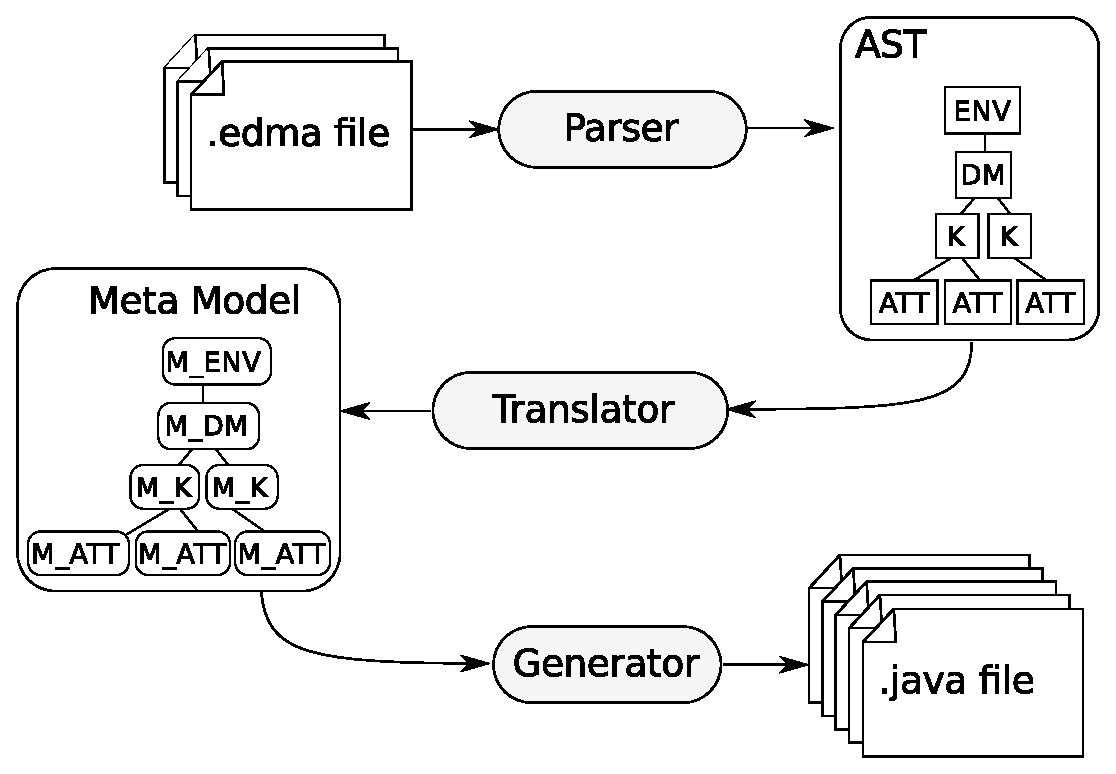
\includegraphics[scale=0.5]{img/compilation.pdf}
	\caption{The compilation of EDMA data definition files is done in three steps: parsing, compilation into a meta model, and generation of Java files.}
	\label{fig:compilation}
\end{figure}

A parser takes in one or many data model definition files with the
extension \texttt{.edma}. While parsing the files, an abstract syntax
tree (AST) representing the data models, is being created. The translator
translates the AST into a meta model, which can then be fed to the
generator. The generator is responsible for outputting Java classes
and interfaces, reflecting the user's data model definition.

It is worth noting, that the abstract syntax tree defines the logical
structure of our environment and data models. The important feature
of the AST is that it makes the translator completely independent
of the concrete textual syntax used in the EDMA language. Having the
AST makes it easy to change the textual grammar and create other syntaxes,
and even create other types of syntaxes. For example, it would be
possible to implement a graphical user interface for drawing data
models, thus serving as a syntax.


\subsubsection{Parser}

For defining the grammer of the textual syntax, we have used a parser
/ scanner generator known as JavaCC. From a JavaCC-grammer, a Java-based
top-down LL(k) parser is generated. The grammar specification is a
variation of EBNF, mixed with Java code for building an instance of
the AST.


\subsubsection{Translator}

The translator takes an AST representing the data model definition,
and creates a meta model instance. The meta model instance can be
seen as an internal representation of the data model definition, and
it is used by both the generator, and by the EDMA runtime system.

When the translator has got a complete AST from the parser, resembling
the user's data model, it does two things. First, it checks whether
everything is consistent within the AST. Then, it simply translates
the AST instance into a Meta Model instance.


\subparagraph{AST Consistency}

In the grammar, syntactical rules governing the data model definition
are specified. However, even if the language is only a data definition
language, there are also some semantic rules, that we must enforce.
Before translating the AST into a meta model, the translator checks
for the presence of circular extensions, unknown references, invalid
ranges in constraints, and value domain loops.
\begin{description}
\item [{Circular~Extensions}] -- The kinds Person and Student could be
defined to extend each other. Instantiation of either would require
an instance of the other to exist. Therefore, we prohibit the user
from making circular extensions of kinds.
\item [{Unknown~References}] -- Wherever the user has written a reference
to an attribute name or a kind name, it must be checked whether the
given attribute or kind is actually defined.
\item [{Value~Domain~Range~Checks}] -- Since the user can specify ranges
on numerical value domains, we have to check that the ranges supplied
actually make sense. For example having a minimum value that is greater
than the maximum value, should be invalid.
\item [{Value~Domain~Loops}] -- Having immutable value domains may be
tricky for the unaware user. Without any check for loops, the user
would be able to define value domains for which there could never
be a valid value. A value domain A of type Struct, could contain an
attribute b, of type \texttt{B}. Likewise, a value domain B of type
Struct could contain an attribute of type A. This is shown on the
listing below.\\
\begin{lstlisting}
ValueDomain A : Struct {
  b : B
}
ValueDomain B : Struct {
  a : A
}
\end{lstlisting}Since in A, b is not optional, it must be supplied at the instantiation
of A. Similarly, when creating a value of B, a value of A must be
supplied. The user could declare a type of B, and set it to null,
and feed it to A upon creation, but this will make the instantiation
of B fail with a nullpointer exception. Since the user might accidentially
create loops, by having many different inter-related value domains,
we have put a check into the compiler, to make it fail as early as
possible.
\end{description}
As soon as an error has been found in the AST, we print out the problem,
the file name and the line number where the error occurred. Each element
in the AST is created with the file name and line number of the statement,
that was the source of it's creation. Therefore, we can easily print
it out when an error occurs in the compilation stage.

After the meta model has been created, the compiler invokes the Generator,
which then starts generating the model-specific Java code.



\subsubsection{Generator\label{sec:Generator}}

The generator is the module responsible for generating Java classes
and interfaces for a specific instance of the meta model.

The generator generates the following:
\begin{itemize}
\item Interfaces and classes for each Value Domain defined in the environment
and the data models.
\item The environment class that contains the instance factories for each
data model in the environment.
\item An instance factory for each data model in the environment, that controls
the individual instances of the data model.
\end{itemize}
For each data model in the environment, the following is generated:
\begin{itemize}
\item The set of interfaces that makes up the internal API, used by the
actions and views to manipulate and view the state of the data model
instance.
\item The set of classes that implements the internal API and binds it to
the runtime interface.
\item The stub classes where the user implements the actions and view. There
is one stub class for each action and view.
\item The external interface for the data model.
\item The implementation of the external interface, that binds the methods
of the interface to the stub classes and execute them through the
runtime interface.
\end{itemize}

\subparagraph{}


\paragraph{\label{sub:Creation-of-values}Value Domains}

The value domains are the type system and infrastructure in EDMA that
binds everything together and ensures that every part of a project
speaks the same language. Each value domain represents a unique type
of data with a well defined structure.

The generator generates two classes for each defined value domain:
An abstract class that serves as an interface to values from the value
domain and an implementation class that implements the abstract methods
in the interface. The reason for using an abstract class instead of
a Java interface is that Java does not support static methods in interfaces
and there are several static methods used to create new values:
\begin{itemize}
\item create - this method creates a new value from scratch 
\item fromString - this method creates a new value from the string representation
of the value.
\item fromStream - this method reads a value from a stream.
\item fromStreamNoValidate - this method reads a value from a stream without
validating it. It should only be used when reading from a trusted
source. For large complex values with many constraints the validate
process could be slow, that is the reason for having this method.
\item fromTerminal - this method uses a terminal to instruct a user to create
a new value.
\end{itemize}
And some abstract methods:
\begin{itemize}
\item toString - returns the string representation of the value.
\item toStream - writes the value to a stream.
\end{itemize}
All value domain classes also have sensible implementations of the
comparable interface, the hashCode and equals methods.

The create method for struct type value domains uses a modified version
of the builder pattern to create new values. The builder pattern uses
what is known as a fluid interface\cite{fowler2008}, where methods
are chained together. This results in more readable code, where each
field has a set-method named after it. In EDMA we have taken the builder
pattern one step further, so each field has its own interface, with
a set-method named after the field. Each set-method then returns the
builder-interface for the next field except the last one, which returns
the created object or value. By doing it this way, we get a fixed
order of the attributes and we make sure that it is not possible to
miss out on any of them. It would be a bit cumbersome to program this
by hand, but with auto-generated code it is no problem. As an example,
lets see how we would create a new date from the date value domain:

\begin{lstlisting}[language=java,frame=none]
Date myDate = Date.create().year(1973).month(6).day(7);
\end{lstlisting}The static method \texttt{Date.create()} returns an interface that
only has a method for setting the year. That method returns an interface
with a method to set the month, which in turn returns an interface
to set the day. The interface for setting the day finally returns
the completed data value. If we put the attributes in a wrong order
or if we missed out any of them, then the Java compiler would complain
immediately. If the user uses a modern IDE e.g. eclipse, it gets very
easy since the automatic code-completion will pop up with the name
of the next field after each dot. This type of chained interfaces
are used in EDMA both when creating values from value domains and
when creating entities from kinds.


\paragraph{Data Models}

For each data model in the environment, several interfaces and classes
are created:
\begin{itemize}
\item Data model factory interface. This interface provides methods to create
new instances of the data model and to get access to existing instances
of the data model. Each instance is identified by a name.
\item Data model instance interface. This interface is used to start and
stop the instance and to get the external interface of the instance.
The methods of the external interface can only be called when the
instance is running. Otherwise an exception is thrown.
\item Data model external interface. This is the external interface of the
data model that clients can use to execute the actions and views on
the data model.
\item Internal view interface. This is the interface that \emph{views} use
internally to navigate and extract information from the data model.
\item Internal update interface. This interface extends the internal view
interface and adds functionality to make changes to the data model.
This is the interface that \emph{actions} use internally.
\end{itemize}
Besides these interfaces there are also generated classes that bind
these data model specific interfaces to the general runtime interface.


\paragraph{Kinds}

For each kind in the data model we create a number of interfaces that
can be used internally in the implementation of the views and actions.
These interfaces are:
\begin{itemize}
\item The entity view interface. This interface provides methods to read
the attributes of an entity of this kind. It will also get the methods
that are used to navigate any relations that this kind is part of.
\item The entity update interface. This interface extends the view interface
and adds methods to update the mutable attributes. This interface
will also get methods to create and delete connections with other
entities through the relations that this kind is part of.
\item The set interface. This interface is used to navigate sets of entities
of this kind. It implements the iterable interface and has methods
to create new sets by unions, intersections and subtractions with
other sets of the same kind. It also gets methods to navigate relations
that this kind is part of.
\item The filter interface. This is a simple interface that can be used
to create specialized filters that can be used on sets of entities
of this kind.
\item The kind interface. This interface has methods to get access to all
entities of this kind or a specific entity either by ID or by any
unique index on the kind. It also has methods to get access to specific
sets of entities based on the indexes declared on this kind.
\end{itemize}
For each kind in the data model, the internal view interface for the
data model gets a method to access the kind interface and the internal
update interface gets methods to create new entities and delete entities
of this kind and a method to upgrade a view interface for an entity
of this kind to an update interface. For singletons we only have the
entity view and entity update interface.

The way we update entities is a little special because of the unique
index. Normally we would just make a set method for each mutable attribute
and then these could be used to update entities one attribute at the
time, but this could give problems if there are unique indexes that
span more than one attribute. As an example, lets say we have a person
kind with separate attributes for first name and last name and that
we have a unique index on (firstName, lastName). There exist a person
called ``John Andersen'' and another person called ``Thomas Andersen''.
Lets say we want to change the name of ``Thomas Andersen'' to ``John
Nielsen'', then we would get an UniqueException if we started by
changing his first name to ``John'', because now there would be
two people named ``John Andersen''. To solve this we have made it
possible to update several attributes at once. Instead of doing something
like this:\begin{lstlisting}[language=java,frame=l]
person.setFirstName("John");
person.setLastName("Nielsen");
\end{lstlisting}We instead do like this:\begin{lstlisting}[language=java,frame=l]
person.setFirstName("John").setLastName("Nielsen").save();
\end{lstlisting}Thus, we update both the first name and the last name at the same
time and we will only get an UniqueException if there is another person
named ``John Nielsen''. The \emph{save} method only declares that
it can throw a UniqueException if we actually update an attribute
that is part of a unique index. This is done by a little trick, where
we actually have two different interfaces for updating the attributes,
a \emph{plain} one where the \emph{save} method does \emph{not} throw
a UniqueException and a \emph{unique} one where the \emph{save} method
declares to throw the UniqueException. In the \emph{plain} interface
all set methods on attributes that are not part of a unique index
just return the \emph{plain} interface again, but the set methods
for those attributes that are involved in a unique index returns the
\emph{unique} interface instead. In the \emph{unique} interface all
set methods returns the \emph{unique} interface again. So this does
that as soon as we have ``touched'' an attribute that is part of
a unique index, then the \emph{save} method will declare that it can
throw the UniqueException.

Besides these interfaces there are also generated classes that binds
these data model specific interfaces to the general runtime interface.


\paragraph{Relations}

The relations in the data model add methods to the interfaces for
the kinds participating in the relation. The names of these methods
are dependent on the type of the relation, as well as names and roles
of the participating kinds. For example, having a relation \texttt{StudentEnrollment}
between \texttt{Course} and \texttt{Person} (having the role of \texttt{student})
results in four methods; two in the \texttt{CourseUpdate} interface
(\texttt{addStudent} and \texttt{removeStudent}), one in the \texttt{PersonViewer}
interface (\texttt{asStudentGetCourseSet}) and one in the \texttt{CourseViewer}
interface (\texttt{getStudentSet}). This is visualized in figure~\ref{fig:generatorRelations}.

\begin{figure}[h]
\rule{\textwidth}{.1mm}
\emph{EDMA file:}
\begin{lstlisting}[language=edma,frame=l]
Relation StudentEnrollment Course >-< Person:student
\end{lstlisting}
\emph{Generated Java:}
\begin{lstlisting}[language=java,frame=l]
public interface CourseUpdater {
	boolean addStudent(PersonViewer student);
	boolean removeStudent(PersonViewer student);
	. . .
}
public interface PersonViewer {
	CourseSet asStudentGetCourseSet();
	. . .
}
public interface CourseViewer {
	PersonSet getStudentSet();
	. . .
}
\end{lstlisting}
\rule{\textwidth}{.1mm}
\caption{Top: The relation as represented in the data definition language. Bottom: The generated code.}
\label{fig:generatorRelations}
\end{figure}Notice that the method in the course viewer interface is not named
\texttt{asCourseGetStudentSet}, but just \texttt{getStudentSet.} Methods
in the \texttt{PersonUpdate} interface for adding and removing courses
(as a student) could be generated as well; however, these would be
redundant with the \texttt{addStudent} and \texttt{removeStudent}
in the \texttt{CourseUpdater} interface. Therefore, the generator
only creates connection methods on the first kind in the relation
(the kind written to the left in the relation declaration).

In a one-to-many relation, a method returning a set of the other kind,
is created on the first kind, while a method returning a single entity
is created on the second kind. This is shown in figure~\ref{fig:generatorRelationsManyOne}.

\begin{figure}[h]
\rule{\textwidth}{0.1mm}
\emph{EDMA file:}
\begin{lstlisting}[language=edma,frame=l]
Relation TeacherAssignment Course >-- Person:teacher
\end{lstlisting}
\emph{Generated Java:}
\begin{lstlisting}[language=java,frame=l]
public interface PersonViewer {
	CourseSet asTeacherGetCourseSet();
	. . .
}
public interface CourseViewer {
	PersonViewer getTeacher();
	. . .
}
\end{lstlisting}
\rule{\textwidth}{0.1mm}
\caption{In a many-to-one relation, a method returning a set is generated on the one-part, while a method returning a single viewer is generated on the many-part.}
\label{fig:generatorRelationsManyOne}
\end{figure}In the \texttt{CourseUpdate} interface, a method is generated for
creating and deleting connections, as shown below.\begin{lstlisting}[language=java,frame=l]
PersonViewer setTeacher(PersonViewer teacher);
\end{lstlisting}This method returns the previous teacher, or \emph{null} if there
previously was no teacher assigned to the course. To remove the current
teacher without setting a new, this method can be called with \emph{null}
as argument.

\begin{figure}[h!]
\rule{\textwidth}{0.1mm}
\emph{EDMA file:}
\begin{lstlisting}[language=edma,frame=none]
Relation Marriage Person:spouse --- Person:spouse
\end{lstlisting}
\emph{Generated Java:}
\begin{lstlisting}[language=java,frame=none]
public interface PersonViewer {
	PersonViewer asSpouseGetSpouse();
	PersonViewer asSpouseSetSpouse(PersonViewer spouse);
	. . . 
}
\end{lstlisting}
\rule{\textwidth}{0.1mm}
\caption{In a one-to-one-self relation, a getter and setter method is generated as expected.}
\label{fig:generatorRelationsOneToOneSelf}
\end{figure}The one-to-one-self relation generates code as expected. Figure~\ref{fig:generatorRelationsOneToOneSelf}
shows a one-to-one-self relation, \texttt{Marriage}, relating two
persons, each with the role of \texttt{spouse}. In the resulting PersonViewer
interface, a method to get the spouse, as well one to set the spouse,
is generated.


\paragraph{Indexes}

There are three types of indexes in EDMA\emph{ (Unique}, \emph{Equal}
and \emph{Compare}) and each of these can be placed both on kinds
and on relations. When an index is placed on a kind, the methods related
to the index are added to the kind's interface. When an index is placed
on a relation, the methods are added to the entity viewer interface.
A Unique index does not only add extra methods to these interfaces,
it also adds a ``\texttt{throws UniqueException}'' declaration to
every method that might violate the unique constraint.

\begin{figure}[h]
\rule{\textwidth}{.1mm}
\emph{EMDA file:}
\begin{lstlisting}[language=EDMA, frame=none, tabsize=4]
Kind Person
{
	name : Name
	email : Email
	birthdate : Date
	Unique(email)
	Compare(birthdate)
}
\end{lstlisting}
\emph{Generated Java:}
\begin{lstlisting}[language=java, frame=none, tabsize=4]
public interface PersonKind {
	PersonViewer getFromID(PersonID id);
	PersonSet getAll();
	
	PersonViewer getFromEmail(Email email);
	PersonSet getWhereBirthdayEquals(Date date);
	PersonSet getWhereBirthdayLessThan(Date date);
	PersonSet getWhereBirthdayLessThanOrEqual(Date date);
	PersonSet getWhereBirthdayGreaterThan(Date date);
	PersonSet getWhereBirthdayGreaterThanOrEqual(Date date);
	PersonSet getWhereBirthdayInRange(
			Date minBirthday, 
			boolean minInclusive,
			Date maxBirthday,
			boolean maxInclusive);
}
\end{lstlisting}
\rule{\textwidth}{.1mm}
\caption{empty}
\label{fig:empty}
\end{figure}


\paragraph{Actions and Views}

Actions and views are the transactions in EDMA. For each Action or
View defined by a data model, a corresponding Java class is created
by the generator. These classes are the placeholders for the Java-code
that makes up the specific action or view. This is best illustrated
by an example: In the data model definition we define an action like
this:

\begin{lstlisting}[frame=l,breaklines=true]
Action createPerson
{
	Description:
		"Creates a new person"
	Input: 
		name : Name,
		email : Email,
		mobile : Mobile
	Output:
		id : PersonID
	ErrorCodes:
		1 - "Email already exists",
		2 - "Mobile already exists"
}
\end{lstlisting}

The generator will then generate the following java class:

\begin{lstlisting}[language=java,frame=l,breaklines=true]
...
public class CreatePersonUserImpl extends 
	Result implements CreatePersonResult
{
	private static final int OK = 0;
	private static final int EMAIL_ALREADY_EXISTS = 1;
	private static final int MOBILE_ALREADY_EXISTS = 2;
	private final Name in_name;
	private final Email in_email;
	private final Mobile in_mobile;
	private PersonID out_id;

	/**
	 * Constructor
	 * @param in_name    Input parameter 1
	 * @param in_email   Input parameter 2
	 * @param in_mobile  Input parameter 3
	 */
	public CreatePersonUserImpl(Name in_name, 
			Email in_email, 
			Mobile in_mobile)
	{
		this.in_name = in_name;
		this.in_email = in_email;
		this.in_mobile = in_mobile;
		out_id = null;
	}

	/**
	 * Execution of the action
	 * @param upd  Update interface
	 * @return     Return 0 to commit or one of the error codes to roll back
	 */
	public int execute(CourseRegUpdater upd)
	{
		// Implementation of createPerson
		// Return one of the following error codes:
		// OK
		// EMAIL_ALREADY_EXISTS
		// MOBILE_ALREADY_EXISTS
		
		// If an error needs extra explanation,
		// use: setErrorDescription("Extra info");
		
		// WARNING : Any code outside the following begin and end tags
		// will be lost when re-generation occurs.
		
		// EDMA_non-generated_code_begin
		
		//TODO : put your implementation here...
		throw new RuntimeException("This action has not been implemented yet!");
		
		// EDMA_non-generated_code_end
	}

	/**
	 * Returns the output id:PersonID
	 * @return  The output id:PersonID
	 */
	public PersonID getId()
	{
		if(errorCode() != 0) return null;
		return out_id;
	}
}

\end{lstlisting}

The user must now implement the business logic that makes up the action
using the interface provided as a parameter in the execute method.
The execute method must return one of the error-codes or 0 (OK) if
successful. The implementation could look like this:

\begin{lstlisting}[language=java,frame=l,breaklines=true]
...
	// EDMA_non-generated_code_begin
	if(upd.getPersonKind().getFromEmail(in_email) != null)
	{
		return EMAIL_ALREADY_EXISTS;
	}
	if(upd.getPersonKind().getFromMobile(in_mobile) != null)
	{
		return MOBILE_ALREADY_EXISTS;
	}
	
	PersonUpdater person = upd.newPerson()
		.name(in_name)
		.email(in_email)
		.mobile(in_mobile)
		.balance(NotNegInt.create(0));
	out_id = person.getID();
	return OK;
	// EDMA_non-generated_code_end
...
\end{lstlisting}

The EDMA framework will take care of calling the execute method and
automatically roll back changes in the case of an error code different
than 0 (OK) is returned or an exception is thrown.

For a view it is almost the same except that the interface provided
as a parameter to the execute method is a ``view'' interface which
means that it has no methods for updating the data model instance.


\paragraph{Utilities}

Because of the fine grained value domain system with well defined,
but arbitrary complex values and the meta description of both the
internal structure and the external interface of the data models,
it is possible to auto-generate many useful utilities for working
with specific data models. This is where the full strength of the
model driven approach comes to play. We have created a few simple
examples of what can be auto generated, but only ones imagination
limits the possibilities of what could be auto generated.

When a new utility has been invented and generation code written,
all both earlier and future projects can benefit from a specialized
version of the utility by the press of a button.


\subparagraph{Remote access}

The generator creates a Java-interface from the actions and views
on each data model defined. This interface is the external interface
to an instance of that data model. This interface will be used by
the client programs that operate on the specific data model instance.
These client programs could be placed within the same JVM as the Data
model instance, but they could also be placed in a different JVM,
perhaps on a different machine. Therefore the generator will generate
a server program and a client proxy that communicates over sockets.
This makes it very easy to separate the client application from the
data model instance if this is needed.

\begin{figure}[h!]
\centering
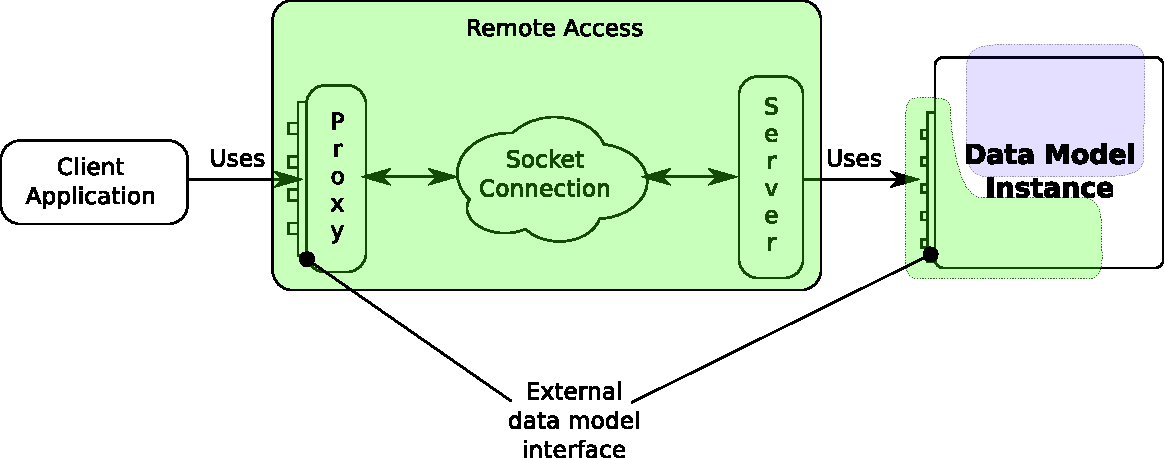
\includegraphics[scale=0.5]{img/remoteAccess.pdf}
\caption{A data model proxy interface and server is generated, to support transparent remote access to a data model instance. Coloured areas are auto generated code.}
\label{fig:remoteAccess}
\end{figure}


\subparagraph{Terminal test}

The generator also generates a program where a user can call the methods
of the external interface through a simple terminal.

\begin{figure}[h!]
\centering
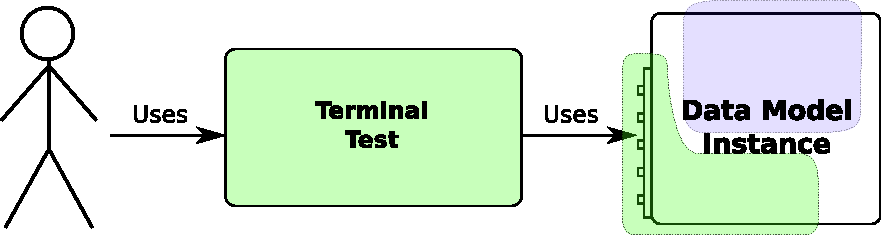
\includegraphics[scale=0.5]{img/terminalTest.pdf}
\caption{An terminal test program is generated to let a user test the methods in the external interface of a data model instance.}
\label{fig:terminalTest}
\end{figure}


\subparagraph{Web Interface}

It would also be possible to generate a web interface where a user
can interact with a data model instance through the external interface.
Javascript can be created to validate the value domains. We have created
an early prototype of this, but it requires a bit more work to be
perfected.

\begin{figure}[h!]
\centering
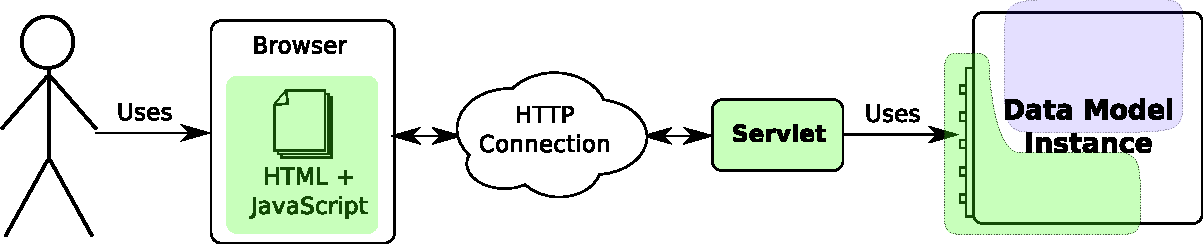
\includegraphics[scale=0.5]{img/web.pdf}
\caption{A web servlet for interacting with a data model instance together with HTML and Javascript for validating values on the client side, could be auto generated.}
\label{fig:web}
\end{figure}


\paragraph{Names and Packages}

It is important to us that the generated code can compile right away
without any changes, so we need to keep track of all imports and package
information. Since many of the generated interfaces and classes are
dependent on each other and on the runtime interface, any changes
to the naming conventions or the package structure would require lots
of changes to the generator code in many different places. To avoid
this we have abstracted out the naming conventions and the package
structure to a separate interface that takes care of all class names,
package names and package layout. This interface is then used all
over the generator. In this way it is easy to make changes to the
names of interfaces and classes or to the package structure of the
generated code. It is even possible to have several implementations
of the naming interface, so it is possible to switch between different
naming and package layout strategies.



\subsection{\label{sec:Runtime}Runtime System}

The runtime system is the module that is responsible for managing
all the data in a data model instance at runtime. This includes the
following tasks:
\begin{itemize}
\item \textbf{Data Containment: }Holding data that make up the current state
of a running data model instance, which includes all entities and
connections between entities.
\item \textbf{Index Containment:} Keeping and updating all indexes on the
data model instance.
\item \textbf{Transaction Execution:} Making sure that all transactions
are executed correctly.
\item \textbf{Data Persistence:} Taking care of the persistence of the data
model instance. 
\end{itemize}
The runtime implements a series of runtime interfaces, used by the
generated code. There could be many different implementations of the
runtime interface, each with different strategies and solutions on
how to solve these tasks. This way it is easy to switch between different
runtime implementations without any changes to the generated code,
or to the code written by the users.


\subsubsection{Runtime Interface}

In the creation of the runtime interface we have tried to make it
independent of how it would be implemented.

Since the runtime interface is non-generated code, it has no knowledge
of specific data models at compile time. It gets the information about
the specific data model that it should manage from the meta model
instance at runtime. Thus, in the runtime interface specific kinds,
relations and indexes are referred to by their index in the meta model
instance.

The runtime interface consists of a number of Java interfaces that
a runtime implementation must implement. These interfaces are:
\begin{itemize}
\item \texttt{IRuntimeFactory} - Given the meta model instance for a specific
data model it returns an \texttt{IDataModelInstanceFactory}
\item \texttt{IDataModelInstanceFactory} - Can load, create and delete individual
instances of a data model.
\item \texttt{IDataModelInstance} - Represents an instance of a data model.
Has methods to start and stop the instance and execute views and actions.
\item \texttt{IView} - Represents a view on the data model implemented by
the user.
\item \texttt{IAction} - Represents an action on the data model implemented
by the user.
\item \texttt{IResult} - Represents the result of executing a view or an
action on the data model instance.
\item \texttt{IDataModelView} - This is the interface that the user implementations
of actions are bound to through the auto-generated internal API interfaces
and classes.
\item \texttt{IDataModelUpdate} - This is the interface that the user implementations
of views are bound to through the auto-generated internal API interfaces
and classes.
\item \texttt{IIndex} - Represents an index on the data model.
\item \texttt{IEntity} - Represents an entity in the data model.
\end{itemize}
Any implementation of an EDMA runtime system must provide these interfaces
for the generated code to bind up against.


\subparagraph{Procedural vs Declarative Query Languages}

In EDMA queries to the data models are written in a procedural manner,
where the user describes an algorithm for how to construct the result,
using the structure of the data model to navigate and using set operations
to narrow or widen the result.

In SQL, queries are written in a declarative way, where the user describes
what the result should be, but not how to obtain it.

It is a subjective matter which of these approaches that feel most
natural, but if a user has an object oriented background, he is used
to get things done in a procedural manner.

One advantage of the declarative approach is that the underlying system
has freedom to analyze the query and try to find the most optimal
algorithm for creating the result.

But even though EDMA takes a procedural approach to obtain the result,
we can use abstraction to let the runtime system delay decisions and
do some amount of optimization on its own. One example of this is
the way sets and set operations are handled in the runtime system.


\subparagraph{Sets and set operations}

One of the important features the runtime system most provide is set
operations such as union, intersection and subtraction. But instead
of representing a set by a java class, we simply use an index that
the runtime system controls. In this way when the user asks the runtime
system to perform an intersection of two sets, all the runtime system
actually gets are the indexes of the sets to intersect and it returns
a new index that represents the intersection of the sets. But the
runtime does not actually have to perform the intersection at this
time. Only when the user actually wants to access or count the elements
in the set, the runtime must perform the intersection. In the case
of complicated queries that involves many set operations before the
final result is produced, the runtime system can analyze and optimize
how to perform these set operations. This method of postponing evaluation
until the result is actually used is known as lazy evaluation.

Especially in a runtime implementation that is backed by an SQL database,
the lazy evaluation is important to avoid sending lots of small queries
to the DBMS, but instead build a larger query behind the scene and
send it when the result is needed. This will both minimize communication
with the DBMS and give the DBMS better optimization opportunities.


\subparagraph{Value domains in the runtime}

Each value domain has its own handler in the meta model instances.
These value domain handlers take care of everything that has to do
with values. To the runtime system a value is simply a Java object
and every time the runtime system needs to do something with a value
(e.g. write it to a stream) it simply invokes the handler for that
specific value domain.


\subsubsection{Example Runtime System}

We have created an example runtime system that are written entirely
in Java. It stores the current state of the data model instances in
memory using standard Java collections like HashMap, HashSet, TreeMap,
TreeSet etc. This gives us a fairly fast implementation but with a
significant memory footprint.


\paragraph{Data Containment}

All the data of a running data model instance, is held in containers
called \emph{Kind Store, Relation Store} and \emph{Index Store}. They
contain all the data that is currently in the data model, as well
as uncommitted data.


\subparagraph{Kind Store}

Entities of any kind are stored in a Kind Store. There is one kind
store for each kind in the data model definition. A kind store is
backed by a hashmap, with a \texttt{Long} as key, and an \texttt{Entity}
object as value. The \texttt{Entity} object contains an object array,
holding the attribute values of the entity.


\subparagraph{Relation Store}

The relation store is used for storing connections between entities.
We have different Relation Store implementations based on cardinality
of the relation. Each end of the relation has a map that maps from
IDs to connected IDs. If the opposite end is a \emph{one} single IDs
are stored as values, if the opposite end is a \emph{many}, sets of
IDs are the values. Special implementations take care of removing
redundancy in self-relations by sorting the IDs before a connection
is inserted or retrieved. 


\paragraph{Index Containment}

As earlier mentioned, EDMA provides three types of indexes on kinds
and on relations: unique, compare and equals. In the example runtime
system the equals- and unique indexes are backed by hashmaps, and
the compare index is backed by a treemap using the NavigableMap interface.

Updates on the indexes are performed whenever a relevant entity is
created, deleted or relevant attributes are updated.


\paragraph{Transaction Execution}

The execution model is responsible for managing the execution of the
transactions. The execution model must ensure the ACID properties.

There are basically two ways of executing transactions. Either, transactions
can be executed sequentially, or they can be executed in parallel.
In most database systems, transaction execution is done in parallel,
using concurrency control mechanisms to secure data integrity. When
executing transactions in parallel, certain concurrency control mechanisms
are needed to ensure the isolation property. Concurrency control can
either be pessimistic or optimistic. 


\subparagraph{Pessimistic Concurrency Control}

In a pessimistic concurrency control mechanism, transactions acquire
locks on data, before they execute. In EDMA, the user writes the transactions
in pure Java, after the code has been generated. This means that EDMA
is not compiling or reading the user created transactions. This makes
it impossible for EDMA to know which parts of the data model the user
is accessing, and hence which parts should be locked.


\subparagraph{Optimistic Concurrency Control}

In the optimistic approach, all reads of a transaction are logged,
and the writes are done to a local cache only, until the commit phase.
In the commit phase it is checked that none of the reads has changed
before the writes are made permanent. If any of the reads has changed,
the entire transaction is canceled and re-executed at a later time.

It would be possible to implement a similar strategy in an EDMA runtime
system, but we have chosen not to do so in the example runtime system
because of: 1) The complexity of it, and the time it would take to
implement, 2) the bookkeeping overhead it would impose, and 3) it
would require that all transactions could risk to be canceled and
re-executed, which puts some heavy constraints on the side effects
that would be allowed inside a transaction. In Java it would be very
hard (if not impossible) to detect and warn about such unwanted side
effects and therefore this would break the illusion that a data model
instance is just a synchronized object.


\subparagraph{Sequential Execution}

The simplest way of obtaining 100\% ACID properties would be to execute
and persist all transactions completely sequentially. Although this
approach would probably be sufficient in many cases where performance
is not a big issue, we can easily get a better performance in a multi-threaded
environment by some parallelization of the process. There are two
ways we can parallelize the process without adding any significant
concurrency control overhead. The first one is to pipeline the process
into an execution step and a persistence step. The second way is to
parallelize views. 

In EDMA, we have chosen to make the actions run sequentially. However,
the sequential run has been pipelined into a two-step process: execution
and persistence. By having the process broken up in two independent
steps, one thread can run the execution of a transaction while another
thread runs the persistence of a previously executed transaction.


\subparagraph{Pipelining}

By pipelining the execution and the persistence, we do not have to
wait for a transaction to be persisted before we can start executing
the next one. Figure~\ref{fig:executionPipelineSimple} illustrates
the idea, representing the different transactions of threads by boxes
in different colors (each color belongs to one thread.)

\begin{figure}[h]
\centering
\subfloat[Simple execution pipeline, with an execution step and a persistence step. Each colored box represents a transaction. Each column represents a distinct time slice.] {\label{fig:executionPipelineSimple1}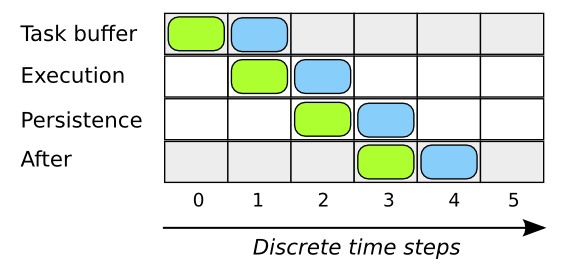
\includegraphics[width=0.5\textwidth]{img/executionPipelineSimple1.png}}\\
\subfloat[Here the persistence step blocks the execution step from fetching in new tasks to execute.]{\label{fig:executionPipelineSimple2}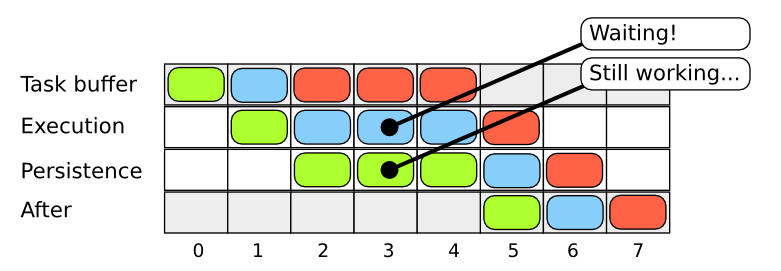
\includegraphics[width=0.7\textwidth]{img/executionPipelineSimple2.png}}
\caption{A simple pipeline helps parallellizing execution and persistance. However, blocking may occur.}
\label{fig:executionPipelineSimple}
\end{figure}In figure \ref{fig:executionPipelineSimple1} a thread starts a transaction,
represented by the green box, at time 0. At time 1, the execution
unit takes the green transaction from the task buffer, and executes
it, while another thread (blue) puts another transaction into the
task buffer. At time 2, the green transaction is handed over to the
persistence unit, while the blue transaction is going into the execution
unit. Now, we can have one thread doing the execution, while another
thread does the persistence. We still return control to the client,
only when the action called by the client has been persisted. Therefore,
the thread issuing the green transaction is blocked, until the green
transaction enters the After slot (only shown for pedagogical reasons).

Each of the two steps in the pipeline are sequentially executed, and
therefore the slowest of them decides the throughput of the complete
pipeline. However, if we add a buffer between the two steps, we can
smooth out the workload of each step, if some transactions are heavier
on the execution and others are heavier on the persistence. The goal
is to keep both the execution and the persistence mechanism as busy
(i.e. non-idling) as possible, with a minimum of waiting. This is
shown on figure~\ref{fig:executionPipelineBetter}. 

\begin{figure}
\centering
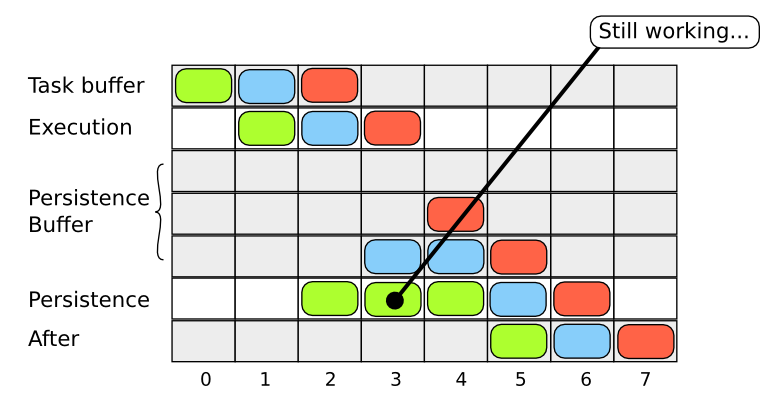
\includegraphics[width=0.7\textwidth]{img/executionPipelineBetter.png}
\caption{By adding a buffer between the execution step, and the persistence step, we can to some extend eliminate blocking of the pipeline.}
\label{fig:executionPipelineBetter}
\end{figure}


\subparagraph{Parallelization of Views}

The second parallelization method takes advantage of the distinction
we have made between the two types of transactions: \emph{actions}
and \emph{views. }Since we know that views can never change the state
of the data model it is safe to parallelize these. It is important
to notice here that even though views have nothing to persist, we
still need to send them through the entire pipeline and not let them
return control to the client thread before they have reached the persistence
step. The reason for this is the \emph{durability} property that we
wish to maintain. We do not want a view to reflect anything in the
data model that has not yet been persisted. If we let the views return
immediately after the execution step, we could get into a situation
where the view reflected the effect of an action that were still in
the persistence buffer, waiting to be persisted. If the persistence
of the action somehow failed, then the view would reflect a non-persisted
state of the data model. Therefore, execution of views is parallelized,
but views must sequentially pass through the persistence unit (which
then does nothing else than marking the view as persisted.)


\subparagraph{The execution algorithm used in the example runtime system}

In EDMA the executor and the persistence module are run in two separate
threads. \emph{Actions} are executed sequentially in the executor
thread while \emph{views }are executed in parallel in their client
threads. The executor has two modes: action-mode and view-mode. When
in action-mode it executes actions in sequence. When in view mode
it lets views execute in their client thread in parallel. When it
switches from view-mode to action-mode, it waits for all current running
views to finish their execution before it starts executing actions.

The pseudo code for the main loop of the executor can be seen in algorithm~\ref{alg:Execution-main-loop}.

\begin{algorithm}[H]
\begin{lstlisting}[tabsize=4]
loop
	t <- get next task from queue
	if(t is an action)
		if(not in action-mode)
			wait for running views to finish
			set mode to action-mode
		executeAction(t)
	else
		set mode to view-mode
		allow t to execute in client thread
\end{lstlisting}


\caption{\label{alg:Execution-main-loop}Execution main loop}
\end{algorithm}


In the current implementation of the executor, a single FIFO queue
is used for both \emph{actions} and \emph{views}. This provides good
fairness, but if \emph{actions} and \emph{views} are highly interleaved,
in the sense that there are no large groups of \emph{views} that are
not interrupted by \emph{actions}, then we do not get much parallelization.
We could instead have two FIFO queues, one for \emph{actions} and
one for \emph{views.} In that way, it would be possible to parallelize
the views in larger chunks. We could then have an algorithm that would
process \emph{views} until the \emph{view} queue is empty and then
switch to process \emph{actions} until the \emph{action} queue is
empty. In order to avoid starvation we could set a maximum number
of transactions to process before looking to the other kind. It is
important to notice here that although this strategy could lead to
a non-chronological execution of transactions, the chronology would
be preserved within each client thread. This is guaranteed, since
whenever a client is executing a transaction, control is never returned
to the client thread before the transaction has been both executed
and persisted.


\paragraph{\label{sub:Persistence}Data Persistence}

In EDMA the current state of the data model is kept in RAM, which
is a volatile storage that is lost in the case of a power failure,
or any other type of system failures. For many applications it is
crucial to store data in a more persistent way so the state of the
data model can be preserved and regenerated even in the case of a
power failure, system reboots an so on. Sometimes it is enough to
store data on a local hard drive, other times applications need a
more secure persistence where data is stored in several different
places.

In EDMA the persistence module is operated on through a simple interface,
making it possible to have different persistence module implementations,
with different strategies for data persistence. Although there is
currently only one implementation, switching between different persistence
strategies can be made into a matter of changing one line of code
for the user. In the following, we describe the strategy that we have
implemented in this project.

Every time an action is executed in EDMA, it generates a sequence
of primitive operations. If the execution fails for some reason, these
operations are rolled back (as described in section \ref{sub:Transactions})
and nothing is sent on to the persistence module. If the action executes
successfully, the sequence of operations that describe all changes
made to the state of the data model instance, is put into an object
called a \emph{persistence unit}. Besides the sequence of operations,
the persistence unit also has two callback functions, one to call
if the data is successfully persisted and another one to call if the
persistence of the data fails for some reason. This persistence unit
is then handed over to the persistence module and whenever the persistence
module has persisted the data or failed in its attempt to do so, it
will call the corresponding callback function on the persistence unit.

This effectively means that every time an action successfully makes
changes to the state of the data model instance, these changes are
persisted as an atomic unit. So when the need for recovery arises,
these changes can be replayed in sequence to re-generate the state.
This also means that a full history of states of the data model is
preserved and could be re-generated if needed.

It is important to note here, that to honor the durability property,
a persistence unit may never be considered successfully persisted
before all preceding persistence units has also been successfully
persisted. Actually \emph{views} also need to pass through the persistence
module as persistence units although they do not have anything to
persist. The reason for this is that the result of a view is not considered
valid or durable before all preceding actions have been successfully
persisted. If the persistence module fails to persist a persistence
unit, then all succeeding persistence units must also be considered
failed, as shown in Figure~\ref{fig:executionPipelineFailing}.

\begin{figure}[h]
	\centering
	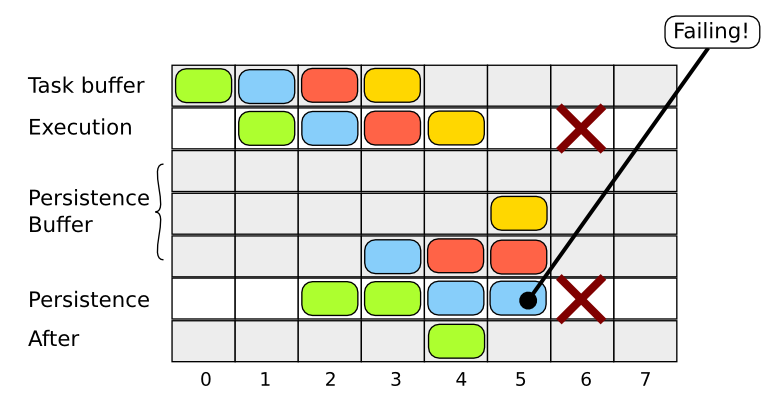
\includegraphics[width=0.7\textwidth]{img/executionPipelineFailing.png}
	\caption{If the persistence module fails, it stops, together with the execution module, and both the task buffer and the persistence buffer is emptied.}
	\label{fig:executionPipelineFailing}
\end{figure}

This may seem like a very bold form of error handling -- shutting
down the whole system, when one thread's transaction fails to be persisted.
However, if the persistence module fails, it means that the disk failed
to write data to the log file, which indicates that there might be
a problem with the disk. Therefore, it wouldn't make sense to continue
writing any subsequent transaction to that file. The failure could
be caused by bad sectors on the disk, which means that it could be
possible to successfully write to a new log file. A clever implementation
of the persistence module (in contrast to our simple proof-of-concept
implementation) could retry writing to the file a number of times,
and upon failure, start writing to a new log file. If that also fails,
writing to another disk could be attempted. Taking it even further,
if writing to any of the disks fails, the system could fall back on
writing to a network socket.

If the system really fails to persist a transaction, EDMA is closed
down, and an administrator will have to manually start the system
again (after running any disk-utility to flag out bad sectors.) Upon
restart, the system reads the whole log file, restoring the data model
to a state identical to the one at the time before the crash.


\subsubsection{SQL Runtime System}

When we planned this thesis, we intended to include a SQL implementation
of the runtime system that would store the data model instances in
a traditional SQL database. 

There are several reasons why this would be a good idea. First, databases
are very mature as a technology, and the database engines are highly
sophisticated and optimized for giving high throughput, serving many
concurrent users, and storing large amounts of data. It would add
some extra work for the user in setting up and connect to a data base,
but this would be rewarded by good scalability in the amount of data
that could be stored. He could always create prototypes with the embedded
java runtime and then switch to the SQL runtime when the need for
storing more data showed up.

However, we chose not to implement an SQL database backed runtime,
because it showed to be more complicated than expected, after we had
invented our value domains system. In an SQL database, there is a
finite set of primitive value domains. In our value domain system,
value domains can be constructed arbitrarily complex, and therefore
there exists an unbounded number of different value domains. This
makes it a non-trivial task to map our entities to SQL tables. It
came to a point where we either had to give up the value domain system
or the SQL implementation due to time constraints.

Given our focus in this project, of investigating the possibilities
of reducing the efforts of coming from a conceptual model to a working
prototype and explore alternative ways of working with data models,
we chose to keep the value domain system and postpone the SQL implementation.


\subsubsection{JDBM3 Runtime System}

The example runtime has the limitation that it can only hold as much
data, as the RAM can contain. Further more, there is a significant
memory footprint in using the example runtime, since all data values
are being wrapped in a number of Java objects, taking up memory (see
the Evaluation section for more details.) For that reason, we have
chosen to exploit the flexibility of the EDMA system, and implemented
the usage of disk-backed sets and maps, using the open source framework
JDBM3. JDBM3 is a key-value store with a number of disk-backed collections,
with the goal of being able to handle billions of items without being
limited by memory. The point of using JDBM3 in EDMA was to have both
large amounts of data, but also to make it possible to perform set
operations on large sets (for results or partial results in actions
and views.)

It turned out that there were some hindrances, making it difficult
to obtain good performance using JDBM3. In order to reach a good performance
level, we need to disable auto-commit in JDBM3. However, having to
manually call commit would require substantial changes in the infrastructure
of the runtime system, therefore complicating the task more than the
benefit added. Further more, it was found that JDBM3 has a bug, preventing
EDMA from using multiple threads access the data store. That said,
since the authors of JDBM3 keep the project alive with frequent updates,
it would be a matter of time before the bug gets fixed.

